% !TeX root = er.tex

\chapter{Movimento de Robôs e Odometria}\label{ch.motion}

Os algoritmos dos capítulos anteriores reagem aos dados dos sensores do robô fazendo com que este mude a velocidade e a direção de seu movimento, mas as mudanças não foram quantitativas. Não exigimos que os robôs se movessem duas vezes mais rápido ou que girassem $90^\circ$ à direita. Os robôs no mundo real têm de se mover para locais específicos e podem ter restrições de engenharia sobre quão rápido ou lento eles podem se mover ou girar. Este capítulo apresenta a matemática do movimento de robôs.

As seções~\ref{s.distance-velocity}--\ref{s.acceleration} revisam os conceitos de distância, tempo, velocidade e aceleração que devem ser familiares da física introdutória. A física do movimento é geralmente ensinada usando cálculo, mas um computador não pode lidar com funções contínuas; em vez disso, devem ser usadas aproximações discretas, como descrito na seção~\ref{s.continuous}.

As seções~\ref{s.odometry}--\ref{s.odometry-turns} apresentam {odometry}, o algoritmo fundamental para computar o movimento de robôs. Uma aproximação da localização de um robô pode ser obtida calculando-se repetidamente a distância movida e a direção de mudança da velocidade das rodas em um curto período de tempo. Infelizmente, a odometria está sujeita a erros graves, como mostrado na seção Sect.~\ref{s.odometry-errors}. É importante entender que os erros de orientação são muito mais significativos do que os erros de distância.

Na implementação mais simples, assume-se que a velocidade das rodas de um robô seja proporcional à potência aplicada aos motores. A seção~\ref{s.wheel} mostra como a precisão da odometria pode ser melhorada com o uso de \emph{wheel encoders}, que medem o número real de rotações das rodas.

A seção~\ref{s.imu} apresenta uma visão geral da \emph{navegação inercial}, que é uma forma sofisticada de odometria baseada na medição da aceleração linear e angular e, em seguida, a integração para obter velocidade e posição. Os sensores para navegação inercial (acelerômetros e giroscópios) já foram muito caros, limitando sua aplicação a aeronaves e foguetes, mas a nova tecnologia chamada \emph{microeletrromecânica} tornou possível a construção de robôs com navegação inercial.

Os carros não podem subir e descer, ao contrário dos helicópteros e submarinos que têm maior liberdade de movimento. Isso se expressa no conceito de \emph{graus de liberdade}, ou \emph{degrees of freedom (DoF)}, em inglês, que é o tema da seção~\ref{s.dof}. A seção ~\ref{s.num-actuators} discute a relação entre o DoF e o número de \emph{atuadores} (motores) em um sistema robótico.

O número de DoF de um sistema não significa que um sistema como um veículo possa se mover livremente em todas essas direções. Um carro pode se mover para qualquer ponto do plano e se orientar em qualquer direção, mas não pode se mover para os lados. Portanto é necessária uma manobra difícil durante o estacionamento paralelo. Isso se deve à diferença entre DoF e o número de graus de mobilidade, ou \emph{Degrees of Mobility (DoM)}, em inglês. Tal assunto é explorado em Sect.~\ref{s.holonomic}, juntamente com o conceito de \emph{movimento holonômico} que relaciona  DoF com DoM.

\section{Distância, Velocidade e Tempo}\label{s.distance-velocity}

Suponha que um robô se mova com uma \emph{velocidade} constante de $10$ cm/s por um período de \emph{tempo} de $5$ s.\footnote{A velocidade é um vetor, portanto possui \emph{amplitude} e \emph{direção}. Um robô pode estar movendo a $10$ cm/s para frente ou para trás; em ambos os casos, a amplitude da velocidade é a mesma, mas sua direção é diferente.}
A \emph{distância} que ele move é de $50$ cm. Em geral, se um robô se move a uma velocidade constante $v$ durante um período de tempo $t$, a distância que ele se move é $s=vt$. Quando potência é aplicada aos motores, faz com que as rodas girem, o que, por sua vez, faz com que o robô se mova a alguma velocidade. Entretanto, não podemos especificar que uma certa potência provoca uma certa velocidade:

\begin{itemize}
\item Nunca dois componentes elétricos ou mecânicos são exatamente idênticos. Um motor é composto de ímãs e fios elétricos cuja interação provoca a rotação de um eixo mecânico. Pequenas diferenças nas propriedades do imã e do fio, assim como pequenas diferenças no tamanho e peso do eixo, podem fazer com que os eixos de dois motores girem a velocidades ligeiramente diferentes para a mesma quantidade de potência.

\item O ambiente afeta a velocidade de um robô. Muito pouco atrito (gelo) ou muito atrito (lama) pode fazer com que um robô se mova mais lentamente em comparação com seu movimento em uma superfície pavimentada seca.

\item Forças externas podem afetar a velocidade de um robô. Ele precisa de mais potência para sustentar uma velocidade específica ao se mover para cima e menos potência ao se mover para baixo, porque a força da gravidade influencia na velocidade. Andar de bicicleta a uma velocidade constante contra o vento exige mais esforço do que andar a favor do vento, e um vento cruzado torna a relação entre potência e velocidade ainda mais complicada.
\end{itemize}

Uma vez que $s=vt$, é suficiente medir quaisquer duas dessas quantidades para calcular a terceira. Se medirmos distância e tempo, podemos calcular a velocidade como $v=s/t$. Distâncias relativamente curtas (até vários metros) podem ser medidas com precisão (até 1 cm) usando uma régua ou uma fita métrica. A aplicação do cronômetro em um smartphone pode medir o tempo com precisão (centésimos de segundo).

\begin{framed}
\act{Velocidade sobre uma distância fixa}{velocity}
\begin{itemize}
\item Escreva um programa que aplique ao seu robô uma mesma potência constante aos seus motores.
\item Marque duas linhas com $1$ m de diferença no chão. Use um cronômetro para medir o tempo que o robô leva para se mover entre as linhas. Calcule a velocidade do robô. Execute o programa dez vezes e registre as velocidades. As velocidades variam?
\item Coloque o robô no chão e execute-o por $5$ s. Meça a distância que ele se move. Calcule a velocidade. Execute o programa dez vezes e registre as velocidades. As velocidades variam?
\item Qual método dá resultados mais precisos?
\item Repita este experimento em diferentes superfícies e discuta os resultados.
\end{itemize}
\end{framed}

A atividade~\ref{act.velocity} mostra que para um ajuste de potência constante, a velocidade de um robô pode variar significativamente. Para navegar com precisão dentro de um ambiente, um robô precisa detectar objetos em seu ambiente, tais como paredes, marcas no chão e objetos.

\section{Aceleração como Mudança de Velocidade}\label{s.acceleration}

A atividade~\ Ref{atividade-fat.velocity} especificou ajustes de potência constantes e, portanto, a velocidade do robô será aproximadamente constante. O que acontece quando a velocidade é variada?

\begin{framed}
\act{Mudança de velocidade}{change-v}
\begin{itemize}
\item Execute o primeiro programa a partir da atividade~\ref{act.velocity} variando a distância entre as marcas: $0,25$ m, $0,5$ m, $1$ m, $1,5$ m, $2$ m. Para cada distância, execute o programa várias vezes e obtenha a média das velocidades calculadas. As velocidades são as mesmas para cada distância?
\item Para melhorar a precisão da medição, coloque marcas no chão a essas distâncias e use o timer do robô para registrar os instantes de tempo em que as marcas são detectadas.
\end{itemize}
\end{framed}

Na atividade~\ref{act.change-v}, você verá que para as distâncias maiores as velocidades estarão próximas umas das outras, mas para as distâncias mais curtas as velocidades serão consideravelmente diferentes. A razão é que a fórmula $v=s/t$ assume que a velocidade é constante ao longo de toda a distância. Na realidade, um veículo deve \emph{acelerar} --mudar sua velocidade-- para passar de uma velocidade zero para uma velocidade constante. Da mesma forma, um veículo deve desacelerar para poder parar.

Para obter uma imagem real do movimento de um robô, precisamos dividir seu movimento em pequenos segmentos $s_1,s_2,ldots$:
\begin{center}
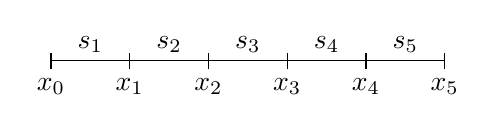
\begin{tikzpicture}
\draw (0,0) -- (5,0);
\foreach \x/\l in {.5cm/$s_1$, 1.5cm/$s_2$, 2.5cm/$s_3$, 3.5cm/$s_4$, 4.5cm/$s_5$}
  \node at (\x,2mm) {\l};
\foreach \x/\l in {0cm/$x_0$, 1cm/$x_1$, 2cm/$x_2$, 3cm/$x_3$, 4cm/$x_4$, 5cm/$x_5$}
  \draw (\x,-1mm) -- (\x,1mm) node[below,yshift=-2mm] {\l};
\end{tikzpicture}
\end{center}
e medir a distância e o tempo para cada segmento individualmente. Em seguida, podemos calcular as velocidades para cada segmento. Simbolicamente, se denotarmos o comprimento do segmento $s_i$ por $\Delta s_i = x_{i+1}-x_i$ e o tempo que o robô leva para cruzar o segmento $s_i$ por $\Delta t_i = t_{i+1}-t_i$, então a velocidade $v_i$ no segmento $s_i$ é dada por:
\[v_i = \frac{\Delta s_i}{\Delta t_i}\,.\]

A Figura~\ref{fig.instant-v} é um gráfico de distância em relação ao tempo para um robô em aceleração. O eixo do tempo foi dividido em segmentos e as inclinações $ \displaystyle \frac{\Delta s_i}{\Delta t_i}$ mostram a velocidade média em cada segmento, que aumenta com o tempo.

\begin{figure}
\begin{center}
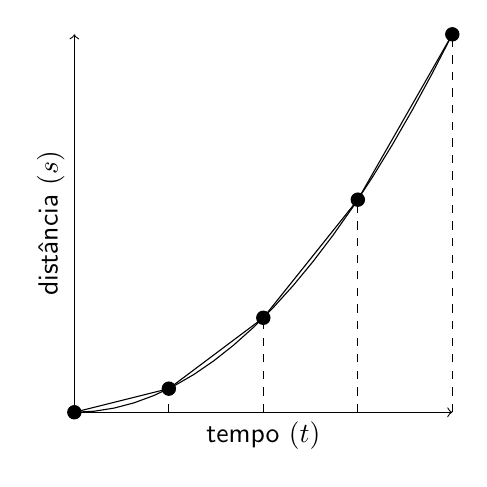
\begin{tikzpicture}[scale=1.2,samples=20,domain=0:4]
\draw[<->] (4,0) -- node[below] {\textsf{tempo} ($t$)} (0,0) -- node[sloped,above] {\textsf{distância} ($s$)} (0,4);
\draw plot (\x,{\x*\x/4});
\draw[mark=*] plot coordinates {(0,0) (1,.25) (2,1) (3,2.25) (4,4)};
\draw[dashed] (1,0) -- (1,.25);
\draw[dashed] (2,0) -- (2,1);
\draw[dashed] (3,0) -- (3,2.25);
\draw[dashed] (4,0) -- (4,4);
\end{tikzpicture}
\caption{Um robô em aceleração: a distância aumenta como o quadrado do tempo}\label{fig.instant-v}
\end{center}
\end{figure}

\emph{A aceleração} é definida como a mudança na velocidade durante um período de tempo:
\[a_i = \frac{\Delta v_i}{\Delta t_i}\,.\]
Quando a potência do robô é ajustada para um valor fixo, a força aplicada ao robô é constante e esperamos que a aceleração permaneça constante, aumentando a velocidade. Entretanto, em determinado ponto a aceleração é reduzida a zero, o que significa que a velocidade não aumenta mais, pois a potência aplicada às rodas é apenas suficiente para superar o atrito da estrada e a resistência do vento.

Vejamos o que acontece se a potência for aumentada com o tempo.

\begin{framed}
\act{Aceleração}{accel}
\begin{itemize}
\item Escreva um programa que faz com que o robô acelere aumentando periodicamente o ajuste de potência. Por exemplo, inicie o robô a $20$ e aumente para $40$ após $1$ s, depois para $60$ após $2$ s, para $80$ após $3$ s e, finalmente, para $100$ após $4$ s.
\item Coloque o robô na pista e execute o programa.
\item Registre as distâncias entre cada mudança da configuração de potência. Calcule e trace as velocidades em cada um desses segmentos.
\end{itemize}
\end{framed}

\section{De Segmentos a Movimento Contínuo}\label{s.continuous}

Na medida em que o tamanho dos segmentos se torna infinitesalmente pequena, obtemos a velocidade instantânea do robô em um único ponto no tempo, expressa como uma derivada:
\[v(t) = \frac{ds(t)}{dt}\,.\]
Da mesma forma, a aceleração instantânea do robô é definida como:
\[a(t) = \frac{dv(t)}{dt}\,.\]
Para aceleração constante, a velocidade pode ser obtida pela integração da derivada:
\[v(t) = \int a\, dt = a\int {dt} = at\,,\]
e então a distância pode ser obtida pela integração novamente:
\[s(t) = \int v(t) dt=\int a\,t\,dt = \frac{at^2}{2}\,.\]

\noindent{}\textbf{Exemplo} Um carro médio acelera de $0$ a $100$ km/h em cerca de $10$ s. Primeiro, nós convertemos unidades de km/h para m/s:
\[
v_{\textit{max}} = 100\, \textrm{km/h} = \frac{100\cdot 1000}{60\cdot 60} \,\textrm{m/s} = 27,\!8 \,\textrm{m/s}\,.
\]
Assumindo aceleração constante, $v_{\textit{max}} = 27,\!8 = a = 10a$, então a aceleração é de $2,\!78 m/s^{2}$ (leia-se, $2,\!78$ metros por segundo por segundo, ou seja, a cada segundo a velocidade aumenta em $2,78$ metros por segundo). A distância que o carro se move em $10$ s é:
\[s(10) = \frac{at^2}{2} = \frac{2,\!78\cdot 10^2}{2}= 139 \,\textrm{m}\,.\]

\begin{framed}

\act{Calculando a Distância Enquanto Acelera}{distance-a}
\begin{itemize}
\item Para vários veículos (carros de corrida, motocicletas), procure o tempo necessário para acelerar de $0$ a $100$ km/h. Calcule a distância percorrida.
\item Assuma que a aceleração de um veículo aumenta linearmente, ou seja, $a=kt$ para um constante $k$. Obtenha $v(t)$ e $s(t)$.
\item Para vários valores de $k$ e $t$, calcule as velocidades e distâncias finais.
\end{itemize}
\end{framed}

\begin{framed}
\act{Medindo o movimento com aceleração constante}{constant-a}
\begin{itemize}
\item Escreva um programa que aplica a configuração de potência máxima a um robô.
\item Coloque o robô sobre uma superfície e execute o programa.
\item Quando o robô atingir sua velocidade máxima, registre o tempo percorrido desde o início da execução.
\item Compare a distância medida com $s = at^2/2$ (Fig.~ ~\ref{fig.acc-distance}).
\item Execute novamente e meça as distâncias em intervalos fixos de tempo. Calcule as velocidades de cada trecho usando as distâncias medidas divididas pelo tempo e compare com $v=at$ (Fig.~\ref{fig.acc-velocity}).
\item Em alguns robôs você pode definir uma velocidade desejada e ler a velocidade real. Se seu robô puder fazer isso, compare as velocidades medidas com as velocidades calculadas.
\end{itemize}
\end{framed}
\begin{figure}
\begin{minipage}{.45\textwidth}
\begin{tikzpicture}[samples=20,domain=0:4]
\draw[<->] (4,0) -- node[below] {\textsf{tempo} ($t$)} (0,0) -- node[sloped,above] {\textsf{velocidade} ($v$)} (0,4) ;
\draw plot (\x,{.5*\x}) ;
\end{tikzpicture}
\caption{Velocidade para aceleração constante}\label{fig.acc-velocity}
\end{minipage}
\hspace{\fill}
\begin{minipage}{.45\textwidth}
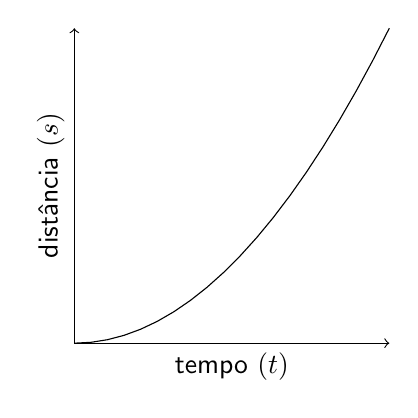
\begin{tikzpicture}[samples=20,domain=0:4]
\draw[<->] (4,0) -- node[below] {\textsf{tempo} ($t$)} (0,0) -- node[sloped,above] {\textsf{distância} ($s$)} (0,4) ;
\draw plot (\x,{.5*\x*\x/2}) ;
\end{tikzpicture}
\caption{Distância para uma aclaração constante}\label{fig.acc-distance}.
\end{minipage}
\end{figure}

%\begin{figure}
%\subfigures
%\begin{minipage}{\textwidth}
%\leftfigure{
%\begin{tikzpicture}[samples=20,domain=0:4]
%\draw[<->] (4,0) -- node[below] {\textsf{time} ($t$)} (0,0) -- node[sloped,above] {\textsf{velocity} ($v$)} (0,4);
%\draw plot (\x,{.5*\x});
%\end{tikzpicture}
%}
%\hspace{\fill}
%\rightfigure{
%\begin{tikzpicture}[samples=20,domain=0:4]
%\draw[<->] (4,0) -- node[below] {\textsf{time} ($t$)} (0,0) -- node[sloped,above] {\textsf{distance} ($s$)} (0,4);
%\draw plot (\x,{.5*\x*\x/2});
%\end{tikzpicture}
%}
%\leftcaption{Velocity for constant acceleration}\label{fig.acc-velocity}
%\rightcaption{Distance for constant accleration}\label{fig.acc-distance}
%\end{minipage}
%\end{figure}

\section{Navegação por odometria}\label{s.odometry}

Suponha que você esteja em um carro e seu sistema de navegação emita a seguinte instrução: ``Em 700 metros, vire à direita''. Agora sua tarefa é muito simples: Faça observações do odômetro do seu carro que mede a distância que você percorreu. Quando seu valor se aproximar de 700 metros além de sua leitura inicial, procure uma rua à direita. Um odômetro em um carro mede velocidade e tempo, e multiplica os dois valores para calcular a distância percorrida.

\emph{Odometria}---a medição da distância---é um método fundamental usado por robôs para navegação. A medição do tempo é fácil usando o relógio interno do computador embarcado. A medição da velocidade é mais difícil: em alguns robôs educacionais, encoders são usados para contar as rotações das rodas (Sect.~\ref{s.wheel}), enquanto em outros a velocidade é estimada a partir das propriedades dos motores. A partir da distância movida $s=vt$, a nova posição do robô pode ser calculada. Em uma dimensão, o cálculo é trivial, mas se torna um pouco mais complexo quando o movimento envolve curvas. Esta seção apresenta o cálculo da distância por odometria, primeiro para um robô movendo-se linearmente e depois para um robô fazendo uma curva.

A seção~\ref{s.odometry-errors} mostra como os erros de orientação são mais sérios do que os erros de distância.

Uma desvantagem da odometria (com ou sem encoders de roda) é que as medidas são indiretas, relacionando a potência dos motores ou o movimento das rodas a mudanças na posição do robô. Isto pode ser sujeito a erros, uma vez que a relação entre a velocidade do motor e a rotação das rodas pode ser muito não-linear e variar com o tempo. Além disso, as rodas podem escorregar e patinar, de modo que pode haver erros ao relacionar o movimento das rodas com o movimento do robô. Estimativas melhoradas da posição podem ser obtidas usando um sistema de navegação inercial, que mede diretamente a aceleração e a velocidade angular que pode ser usada para determinar a posição do robô (Sect.~\ref{s.imu}).

A odometria é uma forma de \emph{localização}: o robô deve determinar sua posição no ambiente. Na odometria, determinamos a posição medindo a mudança a partir da posição inicial conhecida do robô, enquanto a localização (Cap.~\ref{ch.local}) refere-se à determinação da posição de um robô em relação às posições conhecidas de outros objetos, tais como marcos ou faróis.

\section{Odometria linear}

Antes de estudar a matemática da odometria, você deve tentar a seguinte atividade:

\begin{framed}
\act{Distância a partir da velocidade e do tempo}{odometry1}
\begin{itemize}
\item Acione o robô com um ajuste de potência constante durante um período de tempo específico e meça a distância percorrida.
\item Repita a medição várias vezes. A distância é constante? Se não, qual é sua variação percentual?
\item Repita a medição várias vezes para diferentes configurações de potência. A distância medida varia linearmente com o ajuste de potência? A \emph{variação} na medição da distância em várias corridas depende do ajuste de potência?
\item Repita a medição para uma configuração de potência fixa, mas por diferentes períodos de tempo e analise os resultados.
\end{itemize}
\end{framed}

Quando uma relação entre potência do motor e velocidade $v$ é determinada, o robô pode calcular a distância movida usando $s=vt$. Se ele começa na posição $(0,0)$ e se move diretamente ao longo do eixo $x$, então após $t$ segundos sua nova posição é $(vt,0)$.

Esta atividade deve demonstrar que é possível medir a distância por odometria com precisão e exatidão razoáveis. Um veículo autônomo pode usar a odometria para determinar sua posição de modo que não tenha de analisar continuamente os dados de seus sensores para verificar se a rua desejada foi alcançada. Dadas as incertezas de movimento e da estrada, o carro não deve depender apenas da odometria para decidir quando virar, mas o erro não será grande e os dados do sensor podem ser analisados para detectar a curva quando a odometria indicar que o carro está nas proximidades do cruzamento.

A atividade~\ref{act.odometry1} pediu que você medisse a distância percorrida em uma dimensão. Três itens de informação precisam ser computados se o movimento estiver em duas dimensões: o robô tem uma \emph{posição} $(x,y)$ relativa a uma origem fixa, e uma \emph{orientação} $\theta$ - ângulo que indica a direção na qual o robô está apontando\footnote{N. do T.: A orientação do robô é medida em relação ao eixo x.} (Fig.~\ref{fig.pos-head}). O conjunto $(x,y,\theta)$ é chamado de \emph{pose} do robô. Se o robô começa na origem $(0,0)$ e se movimenta em linha reta no ângulo $\theta$ com velocidade $v$ no tempo $t$, a distância movida é $s=vt$. Sua nova posição $(x,y)$ é:
\begin{eqnarray*}
x &=& vt \cos \theta\\
y &=& vt \sin \theta\,.
\end{eqnarray*}

\begin{figure}
\begin{center}
\begin{tikzpicture}[scale=1.2]
\draw (-1,0) -- (4,0);
\draw (0,-1) -- (0,3);
\node at (-5mm,-4mm) { $(0,0)$ };
\pic[rotate=30,scale=.6] at (0,0) { robot };
\pic[rotate=30,scale=.6] at (30:3) { robot };
\draw[dashed] (30:3) -| (0,0);
\draw[dashed] (30:3) |- (0,0);
\node at (1.2,1.7) {$x$};
\node at (2.8,.5) {$y$};
\draw[->] (30:3) -- +(30:1.2) {};
\draw[->] (0,0) -- +(30:1.2) {};
\node at (1,.3) {$\theta$};
\end{tikzpicture}
\caption{Posição e orientação}\label{fig.pos-head}
\end{center}
\end{figure}

\section{Odometria com Curvas}\label{s.odometry-turns}

Suponha que o robô gire ligeiramente para a esquerda porque a roda direita se move mais rápido do que a roda esquerda (Fig.~\ref{fig.small-turn}). Na figura, o robô está orientado para o topo da página; o ponto azul é a roda esquerda, o ponto vermelho é a roda direita, e o ponto preto é o centro do robô que está na metade do caminho entre as rodas. A \textit{linha} $b$ indica a distância entre as rodas, e $d_l, d_r, d_c$ representam as distâncias percorridas pelas duas rodas e pelo centro enquando o robô se move. Queremos calcular a nova posição e orientação do robô após seu deslocamento.

Podemos medir $d_l$ e $d_r$, as distâncias movimentadas pelas duas rodas, usando o método descrito na Actividade~\ref{act.odometry1}: relacionando a potência do motor à velocidade de rotação e depois multiplicando pelo tempo. Alternativamente, podemos usar o número de rotações contadas pelos encoders das rodas. 
\begin{equation}
d_i=2\pi R \omega_i t,\;\;\; i=l,r\,. \label{eq.rotation}
\end{equation}
A tarefa é determinar a nova pose do robô após as rodas terem movido essas distâncias.

\begin{figure}
\begin{center}
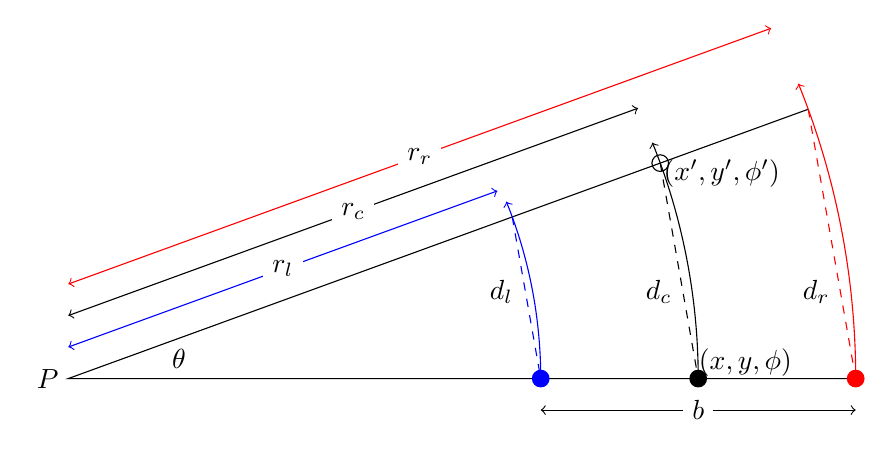
\begin{tikzpicture}
% Draw angle lines
\draw (10,0) -- %
  (0,0) coordinate(origin) node [right=40pt,above] {$\theta$} -- %
  (20:10);
\node[left] at (0,0) {$P$};
% Arrows with baseline
\draw[<->] (6,-.4) -- %
  node[fill=white] {$b$} (10,-.4);
% Three: large dots, arcs, dashed lines, labels
\foreach \x/\d/\c in {6/$d_l$/blue,8/$d_c$/black,10/$d_r$/red}
{
  \draw[dashed,\c] (20:\x) -- (\x,0);
  \draw[->,\c] (\x,0) arc (0:22:\x);
  \node at (\x-.5,1.1) {\d};
  \draw[fill,\c] (\x,0) circle[radius=3pt];
}
\draw[<->,blue] (0,4mm) -- node[black,fill=white] {$r_l$} +(20:58mm);
\draw[<->,black] (0,8mm) -- node[black,fill=white] {$r_c$} +(20:77mm);
\draw[<->,red] (0,12mm) -- node[black,fill=white] {$r_r$} +(20:95mm);
\node at (8.6,.2) {$(x,y,\phi)$};
\node at (8.3,2.6) {$(x',y',\phi')$};
\draw (20:8) circle[radius=3pt];
\end{tikzpicture}
\end{center}
\caption{Geometria de uma curva à esquerda por um robô com duas rodas}\label{fig.small-turn}
\end{figure}

A figura~\ref{fig.small-turn} mostra o robô inicialmente na pose $(x,y,\phi)$, onde o robô está voltado para o norte ($\phi=\pi/2$). Depois de girar $\theta$ radianos, qual é sua nova pose $(x',y',\phi')$? Claramente, a nova orientação do robô é $\phi'=\phi+\theta$, mas também temos de calcular $x',y'$.

O comprimento de um arco de ângulo $\theta$ radianos é dado por sua fração da circunferência do círculo: $2\pi r,(\theta/2\pi)=\theta r$. Para ângulos pequenos, as distâncias $d_l,d_c,d_r$ são aproximadamente iguais ao comprimento dos arcos correspondentes, portanto temos:
\begin{eqnarray}
\theta &=& d_l/r_l = d_c/r_c = d_r/r_r\,,\label{eqn.theta}
\end{eqnarray}
onde $r_l, r_r, r_c$ são as distâncias a partir de $P$, o centro da curva.

As distâncias de $d_l$ e $d_r$ são obtidas a partir das rotações das rodas (Eq.~\ref{eq.rotation}) e a distância $b$ é uma medida física fixa do robô (distância entre as rodas). Da Eq.~\ref{eqn.theta}, pode-se calcular o ângulo $\theta$:
\begin{eqnarray*}
\theta r_r &=& d_r\\
\theta r_l &=& d_l\\
\theta r_r - \theta r_l &=& d_r - d_l\\
\theta &=& (d_r - d_l) / (r_r - r_l)\\
\theta &=& (d_r - d_l) / b\,.
\end{eqnarray*}
O centro fica a meio caminho entre as rodas $r_c =(r_l+r_r)/2$,
novamente a partir da Eq.~\ref{eqn.theta}, tem-se:
\begin{eqnarray*}
d_c&=&\theta r_c\\
&=&\theta \left(\frac{r_l+r_r}{2}\right)\\
&=&\frac{\theta}{2} \left(\frac{d_l}{\theta} + \frac{d_r}{\theta}\right)\\
&=&\frac{d_l+d_r}{2}\,.
\end{eqnarray*}

Se a distância movida for pequena, a linha rotulada $d_c$ é aproximadamente
perpendicular ao raio através da posição final do robô. Por semelhança de triângulos, vemos que $\theta$ é a mudança na orientação do robô (Fig.~\ref{fig.heading}). Por trigonometria:\footnote{Talvez você esperasse ver $\cos$ para $dx$ e $\sin$ para $dy$. Esse seria o caso se o robô estivesse orientado ao longo do eixo $x$. Entretanto, a orientação inicial é de $\phi=\pi/2$, e nós temos $\sin(\theta+\pi/2)=\cos\theta$ e $\cos(\theta+\pi/2)=-\sin\theta$.}
\begin{eqnarray*}
\textit{dx} &=& - d_c \sin \theta\\
\textit{dy} &=& d_c \cos \theta\,,
\end{eqnarray*}
Assim, a pose do robô após seu deslocamento é:
\[
(x',y',\phi') = ( - d_c \sin \theta, d_c \cos \theta, \phi+\theta)\,.
\]

\begin{figure}
\begin{center}
\begin{tikzpicture}
% Draw angle with thetas
\draw (10,0) coordinate (A) -- %
  (0,0) coordinate (origin) node [right=40pt,above] {$\theta$} -- %
  (20:9) coordinate (B) node [xshift=1.5mm,yshift=-7mm] {$\theta$};
% Dashed line to complete the triangle
\draw[dashed] (A) -- node [right=1pt] {$d_c$} (B);
% Dashed perpendicular lines
\draw[dashed] (B) -- node [left] {$d_y$} ({B} |- {A}) coordinate (C);
\draw[dashed] (A) node[above left,xshift=1pt,yshift=14pt] {$\theta$} -- (A |- B);
% Dummy line for placing dx label
\path (C) -- node [below=1pt] {$d_x$} (A);
% Rectangles for right angles
\draw (C) rectangle +(6pt,6pt);
\draw[rotate=20] (B) rectangle +(-6pt,-6pt);
\end{tikzpicture}
\end{center}
\caption{Mudança na orientação}\label{fig.heading}
\end{figure}

As fórmulas mostram como calcular as mudanças \textit{dx}, \textit{dy} e $\theta$ quando o robô se move a uma curta distância. Para computar a odometria em distâncias maiores, este cálculo deve ser feito com frequência. Há duas razões pelas quais os intervalos entre os cálculos devem ser curtos: (a) a suposição de velocidade constante se mantém apenas para distâncias curtas, e (b) o cálculo trigonométrico é simplificado ao supor que a distância movida é curta.

\begin{framed}
\act{Odometria em duas dimensões}{odometry2}
\begin{itemize}
\item Escreva um programa que faça o robô girar suavemente à esquerda por um período de tempo específico.
\item Calcule sua pose $( - d_c \sin \theta, d_c \cos \theta, \theta)$ e compare o resultado com os valores medidos usando uma régua e um transferidor. Execute o programa várias vezes e verifique se as medidas são consistentes.
\item Execute o mesmo programa por diferentes períodos de tempo. Como isso afeta a precisão e a exatidão do cálculo da odometria?
\end{itemize}
\end{framed}

\section{Erros na odometria}\label{s.odometry-errors}

Já observamos que a odometria não é precisa porque medições inconsistentes e irregularidades na superfície podem causar erros. Nesta seção mostramos que mesmo pequenas mudanças na direção do movimento do robô podem causar erros muito maiores do que aqueles causados por mudanças em seu movimento linear.

Para simplificar a apresentação, vamos assumir que um robô deve mover-se por $10$ metros a partir da origem de um sistema de coordenadas ao longo do eixo $x$ e, em seguida, verificar seu entorno em busca de um objeto específico. Qual é o efeito de um erro de até $p\,\%$? Se o erro está na medida de $x$, a distância movimentada, então o erro $\Delta x$ em $x$ é:
\[\Delta x \leq \pm 10\cdot\frac{p}{100} = \pm\frac{p}{10}\; \textrm{meter}\,,\]
onde o valor é negativo ou positivo porque o robô poderia mover-se para uma posição a uma distância $p\,\%$ antes ou depois da posição pretendida.

Suponha agora que exista um erro de $p\%$ na \emph{orientação} do robô, e, para simplificar, suponha que não há erro na distância movida. A geometria é:
\begin{center}
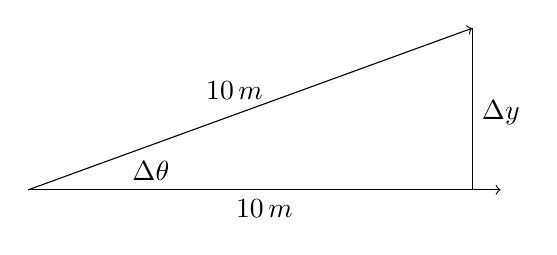
\begin{tikzpicture}
\draw[->] (0,0) -- node[below] {$10\,m$} (6,0);
\draw[->] (0,0) -- node[above,xshift=-2mm] {$10\,m$} +(20:6);
\draw (20:6) |- node[above right,yshift=7mm] {$\Delta y$} (0,0);
\node[above right,xshift=12mm] at (0,0) {$\Delta \theta$};
\end{tikzpicture}
\end{center}
O robô pretendia mover-se por $10$ m ao longo do eixo $x$ mas, em vez disso, moveu-se levemente para a esquerda num ângulo de $\Delta\theta$. Vamos computar o desvio esquerda-direita de $\Delta y$. Por trigonometria, $\Delta y = 10\sin \Delta\theta$. Um erro de $p\,\%$ na orientação é:
\[
\Delta\theta=360\cdot\frac{p}{100}=(3.6p)^\circ\,,
\]
portanto, o desvio esquerda-direita é:
\[
\Delta y \leq \pm 10 \sin (3.6p)\,.
\]

As tabelas a seguir comparam a diferença entre um erro linear (esquerda) de $p\,\%$ e um erro angular (à direita) de $p\,\%$:
\begin{displaymath}
\setlength{\arraycolsep}{2ex}
\renewcommand{\arraystretch}{1.1}
\begin{array}{r|r}
\hline\noalign{\smallskip}
\multicolumn{1}{c|}{p\,\%} & \multicolumn{1}{c}{\Delta x \,(m)}\\
\noalign{\smallskip}\hline\noalign{\smallskip}
1 & .1 \\
2 & .2 \\
5 & .5 \\
10 & 1.00\\
\noalign{\smallskip}\hline\noalign{\smallskip}
\end{array}
\;\;\;\;\;\;\;\;
\begin{array}{r|rrr}
\hline\noalign{\smallskip}
\multicolumn{1}{c|}{p\,\%} & \multicolumn{1}{c}{\Delta \theta\,({}^\circ)} & \multicolumn{1}{c}{\sin\Delta\theta} & \multicolumn{1}{c}{\Delta y \,(\textrm{m})}\\
\noalign{\smallskip}\hline\noalign{\smallskip}
1 &  3,6 & 0,063 & 0,63\\
2 &  7,2 & 0,125 & 1,25\\
5 &  18,0 & 0,309 & 3,09\\
10 & 36,0 & 0,588 & 5,88\\
\noalign{\smallskip}\hline\noalign{\smallskip}
\end{array}
\end{displaymath}

Para um erro muito pequeno como $2\,\%$, o erro de distância após mover $10$ m é de apenas $0,2$ m, o que deve colocar o robô nas proximidades do objeto que está procurando. No entanto, um erro de direção da mesma porcentagem coloca o robô a $1,25$ m de distância do objeto. Para um erro mais significativo como $5\,\%$ ou $10\,\%$, o erro de distância ($50$ cm ou $100$ cm) ainda é possivelmente contornável, mas o erro de orientação coloca o robô a $3,09$ m ou $5,88$ m de distância, que não está nem mesmo nas proximidades do objeto.

O acúmulo de erros de odometria à medida que a distância movida se torna maior é exibida na Fig.~\ref{fig.odo-errors}. A posição inicial do robô é denotada pelo ponto na origem.  Assumindo um erro máximo de $pm 4\,\%$ tanto na direção linear quanto na orientação do robô, as possíveis posições do robô depois de mover-se por $d=1,2,\ldots,10$ metros são exibidas como elipses. Os raios menores das elipses de erro resultam dos erros lineares:
\[0,04s = 0,04, 0,08, \ldots, 0,4 \;\;\textrm{metros},
\]
enquanto os raios maiores das elipses de erro resultam dos erros angulares:
\[
d\sin \,(0,04\cdot 360^\circ)=d \sin 14,4^\circ \approx{} 0,25, 0,50, \ldots 2,5\;\;\textrm{metros}.
\]
Claramente, os erros angulares são muito mais significativos do que os erros lineares.

\begin{figure}
\begin{center}
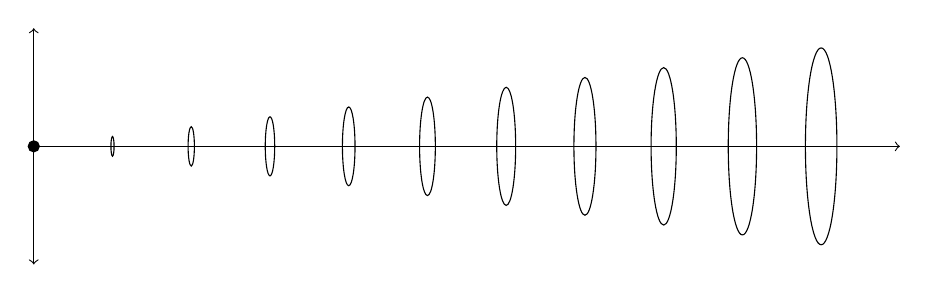
\begin{tikzpicture}
\draw[<->] (0,1.5) -- (0,-1.5);
\draw[->] (0,0) -- (11,0);
\draw[fill](0,0) circle[radius=2pt];
\foreach \x/\mult in {1/1, 2/2, 3/3, 4/4, 5/5, 6/6, 7/7, 8/8, 9/9, 10/10}
  \draw (\x,0) ellipse [x radius=\mult*.02cm, y radius=\mult*.125cm];
\end{tikzpicture}
\end{center}
\caption{Erros de odometria}\label{fig.odo-errors}
\end{figure}

Como o erro é inevitável, periodicamente a pose do robô computada pela odometria deve ser comparada com uma posição absoluta; esta se torna a nova posição inicial para posterior cálculo. Os métodos para determinar a posição absoluta do robô são apresentados no Capítulo~\ref{ch.local}.

\begin{framed}
\act{Erros de odometria}{odo-error}
\begin{itemize}
\item Escreva um programa para fazer o robô mover-se em linha reta por $2$ metros. Certifique-se de que a superfície esteja lisa para que ele não se desvie do curso e calibre as potências dos motores para que o robô se movimente o máximo possível em linha reta.
\item Varie a potência do motor de ambas as rodas juntas para que o robô funcione um pouco mais lento ou um pouco mais rápido do que antes. Trace sua posição em intervalos fixos e veja se o erro permanece linear ao longo da trajetória.
\item Varie a potência do motor de uma roda de modo que o robô gire ligeiramente para um lado. Trace sua posição em intervalos fixos e verifique se os erros são proporcionais ao seno da diferença entre a orientação original e a nova orientação.
\end{itemize}
\end{framed}

\begin{framed}
\act{Efeito combinado de erros de odometria}{odo-combine}
\begin{itemize}
\item Escreva um programa que faça o robô mover-se em linha reta por $2$ metros e depois gire $360^\circ$. Qual é o erro na posição do robô?
\item Escreva um programa que faz com que o robô gire $360^\circ$ e depois se movimente em linha reta por $2$ metros. Qual é o erro na posição do robô? Existe uma diferença entre este erro e o erro da experiência anterior?
\item Escreva um programa que faz o robô mover-se em linha reta por $2$ metros, girar $180^\circ$, e em seguida mover-se em linha reta por mais $2$ metros. A que distância está de sua posição inicial?
\end{itemize}
\end{framed}

\begin{framed}
\act{Correção de erros de odometria}{odo-correct}
\begin{itemize}
\item Modifique o programa que você escreveu para a Activity~\ref{act.odo-error} para introduzir \emph{jitter}, variação aleatória na potência fornecida ao motor. Verifique se a distância que o robô se move em um tempo fixo não é constante, mas muda ligeiramente de corrida para corrida.
\item Marque uma linha de destino no chão e calcule o tempo que o robô deve levar para alcançar tal destino.
\item Execute o programa. Após o período de tempo calculado no item anterior, verifique se o robô pode encontrar a linha movendo-se para frente e para trás em pequenos passos até detectá-la.
\end{itemize}
\end{framed}

\section{Encoders de roda}\label{s.wheel}

A odometria em um veículo com rodas como um carro pode ser melhorada medindo a rotação das rodas ao invés de se inferir sua velocidade a partir da potência aplicada aos motores. A circunferência de uma roda é de $2\pi r$, onde $r$ é o raio da roda (por exemplo, em cm). Portanto, se $n$ rotações forem contadas, sabemos que o robô se moveu $2\pi n r$ cm. Os encoders de roda podem ser construídos para medir as frações de uma revolução. Se um pulso é gerado $8$ vezes por revolução, a distância movida é $2\pi nr /8$ cm, onde $n$ é agora o número de pulsos gerados pelo sensor do encoder.

Há muitas maneiras diferentes de implementar encoders de roda. Um projeto popular é usar uma fonte de luz como um diodo emissor de luz (LED), um sensor de luz e um disco codificador que é anexado ao eixo da roda (Fig.~\ref{fig.wheel}). O disco é perfurado com furos (Fig.~\ref{fig.encoding-disk}) para que o sensor gere um sinal sempre que o furo estiver alinhado com a fonte de luz.

\begin{figure}
\begin{minipage}{.5\textwidth}
\begin{tikzpicture}[scale=.7]
% Draw axle
\draw[thick,fill=gray!80] (0,-.18) rectangle (5,.18) node[right=4pt,yshift=10pt,text width=8mm] {\textsf{ao motor}};
% Draw disk
\draw[rounded corners,fill=gray!10] (3,-1.6) node[right=10pt,yshift=3pt] {\textsf{disco codificador}} rectangle +(.4,3.2);
% Draw wheel
\draw[rounded corners,thick,fill=gray!20] (0,-2) to [bend left=10] (0,2) node[xshift=3.5mm,yshift=3mm] {\textsf{roda}} -- (1,2) to [bend left=10](1,-2) -- cycle;
\begin{scope}[xshift=20mm,yshift=8mm]
% LED
\draw[red] (0,0) rectangle node[black,above=12pt] {\textsf{LED}} (.3,.6);
\draw[red,bend right=90] (.3,0) to (.3,.6);
% Sensor
\draw[blue] (2,0) rectangle node[black,above=12pt] {\textsf{sensor}} (2.3,.6);
\draw[blue,bend left=90] (2,0) to (2,.6);
\end{scope}
\draw[raxis] (-15mm,0) -- (64mm,0);
\end{tikzpicture}
\caption{Encoder óptico de roda}\label{fig.wheel}
\end{minipage}
\hspace{\fill}
\begin{minipage}{.45\textwidth}
\begin{center}
\begin{tikzpicture}[scale=.5,baseline=-14mm]
\draw[fill=gray!20] (0,0) circle [radius=25mm];
\draw[fill=white] (0,0) circle [radius=5mm];
\foreach \x/\y/\theta in {
  0/18/0, 0/-18/0, 18/0/90, -18/0/90,
  12.5/12.5/-45, -12.5/12.5/45, 12.5/-12.5/-135, -12.5/-12.5/135
} {
  \node [draw,fill=white,shape=rectangle,inner sep=0pt,minimum width=3mm,minimum height=5mm,anchor=center,rotate=\theta] at (\x mm,\y mm) {};
}
\draw[raxis] (0,0) -- (10pt,0);
\draw[raxis] (0,0) -- (-10pt,0);
\draw[raxis] (0,0) -- (0,10pt);
\draw[raxis] (0,0) -- (0,-10pt);
\end{tikzpicture}
\end{center}
\caption{Disco codificador}\label{fig.encoding-disk}
\end{minipage}
\end{figure}


%\begin{figure}
%\subfigures
%\begin{minipage}{\textwidth}
%\leftfigure[c]{
%\begin{tikzpicture}[scale=.7]
%% Draw axle
%\draw[thick,fill=gray!80] (0,-.18) rectangle (5,.18) node[right=4pt,yshift=10pt,text width=8mm] {\textsf{to motor}};
%% Draw disk
%\draw[rounded corners,fill=gray!10] (3,-1.6) node[right=10pt,yshift=3pt] {\textsf{encoding disk}} rectangle +(.4,3.2);
%% Draw wheel
%\draw[rounded corners,thick,fill=gray!20] (0,-2) to [bend left=10] (0,2) node[xshift=3.5mm,yshift=3mm] {\textsf{wheel}} -- (1,2) to [bend left=10](1,-2) -- cycle;
%\begin{scope}[xshift=20mm,yshift=8mm]
%% LED
%\draw[red] (0,0) rectangle node[black,above=12pt] {\textsf{LED}} (.3,.6);
%\draw[red,bend right=90] (.3,0) to (.3,.6);
%% Sensor
%\draw[blue] (2,0) rectangle node[black,above=12pt] {\textsf{sensor}} (2.3,.6);
%\draw[blue,bend left=90] (2,0) to (2,.6);
%\end{scope}
%\draw[raxis] (-15mm,0) -- (64mm,0);
%\end{tikzpicture}
%}
%\hspace{\fill}
%\rightfigure[c]{
%\begin{tikzpicture}[scale=.5,baseline=-14mm]
%\draw[fill=gray!20] (0,0) circle [radius=25mm];
%\draw[fill=white] (0,0) circle [radius=5mm];
%\foreach \x/\y/\theta in {
%  0/18/0, 0/-18/0, 18/0/90, -18/0/90,
%  12.5/12.5/-45, -12.5/12.5/45, 12.5/-12.5/-135, -12.5/-12.5/135
%} {
%  \node [draw,fill=white,shape=rectangle,inner sep=0pt,minimum width=3mm,minimum height=5mm,anchor=center,rotate=\theta] at (\x mm,\y mm) {};
%}
%\draw[raxis] (0,0) -- (10pt,0);
%\draw[raxis] (0,0) -- (-10pt,0);
%\draw[raxis] (0,0) -- (0,10pt);
%\draw[raxis] (0,0) -- (0,-10pt);
%\end{tikzpicture}
%}
%\leftcaption{Optical wheel encoder\label{fig.wheel}}
%\rightcaption{Encoding disk\label{fig.encoding-disk}}
%\end{minipage}
%\end{figure}

O suporte para encoders de roda em robôs educacionais varia:
\begin{itemize}
\item Se um robô não tiver encoders de roda, ele deve ser calibrado;
\item O robô pode ter encoders de roda que são usados internamente;
\item Alguns robôs como o \lego Mindstorms permitem que o usuário leia os encoders.
\end{itemize}
A seguinte atividade propõe uma experiência para medir a distância movimentada através da contagem das rotações de uma roda. Ela pode ser realizada mesmo que seu robô não possua encoders de roda, ou que não sejam acessíveis.

\begin{framed}
\act{Encoders de rodas}{wheel}
\begin{itemize}
\item Faça uma marca no topo de uma roda do robô usando giz ou prendendo um pedaço estreito de fita adesiva colorida. Escreva um programa que faça com que o robô se mova para frente durante um período de tempo fixo. Execute o programa e faça um vídeo da lateral do robô usando a câmera de seu smartphone.
\item Veja o vídeo e determine o número de rotações contando o número de vezes que a marca está na parte superior da roda.
\item Meça o raio da roda e calcule a distância movida. Quão próximo está o resultado da distância real medida no chão?
\item Repeta a medição usando $n=2$ e depois $n=4$ marcas igualmente espaçadas na roda. Determine o número de rotações contando o número de vezes que uma marca está na parte superior da roda e divida por $n$. Calcule a distância.
\end{itemize}
\end{framed}

\section{Sistemas de navegação inercial}\label{s.imu}

Um \emph{sistema de navegação inercial (INS, em inglês)} mede diretamente a aceleração linear e a velocidade angular e os utiliza para calcular a pose de um veículo. O termo \emph{inertial measurement unit (IMU)} também é usado, mas preferimos o termo INS, que se refere a todo o sistema. A integração da aceleração desde a pose inicial até o instante atual $\tau$ resulta na velocidade atual:
\[
v=\int_0^\tau a(t) \,dt\,.
\]
Da mesma forma, a integração da velocidade angular resulta no valor de mudança de orientação:
\[
\theta = \int_0^\tau \omega(t) \, dt\,.
\]
Em um INS, funções contínuas de integração não são fornecidas; em vez disso, a aceleração e a velocidade angular são amostradas e a soma substitui a integração:
\[
v_n = \sum^{n}_{i=0} a_n \Delta t,\;\; \theta_n = \sum^{n}_{i=0} \omega_n \Delta t\,.
\]
Os INSs estão sujeitos a erros causados por imprecisões na própria medição, bem como por variações causadas por fatores ambientais, como temperatura, e pelo desgaste da unidade. A medição inercial é frequentemente combinada com GPS (Sect.~\ref{s.gps}) para atualizar a posição com uma localização absoluta.

Os INS para robôs são construídos com \emph{microelectromechanical systems (MEMS)}, que utilizam técnicas de fabricação de circuitos integrados que combinam elementos mecânicos com eletrônicos que fazem interface com o computador do robô.

\subsection{Acelerômetros}\label{s.accelerometer}

Se você já voou em um avião, você já experimentou uma força que o empurrou contra seu assento como resultado da rápida aceleração do avião na decolagem. Ao pousar, você é empurrado para longe de seu assento. Você também pode experimentar isto em um carro que acelera rapidamente ou faz uma parada de emergência. A aceleração está relacionada à força pela segunda lei de Newton $F=ma$, onde $m$ é a massa. Ao medir a força sobre um objeto, podemos calcular sua aceleração.

As figuras~\ref{fig.acc-forward}--\ref{fig.acc-backward} mostram como um acelerômetro pode ser construído a partir de um objeto (\emph{massa}) conectado a uma mola. Quanto maior a aceleração, maior a força exercida pela massa sobre a mola, que por sua vez faz com que a mola seja comprimida. O sentido que a massa se move dá o sinal da aceleração: para frente ou para trás. A magnitude da força é obtida indiretamente medindo-se a distância que a massa se move. Você pode ver que os diagramas correspondem à nossa experiência: quando um carro acelera, você é empurrado de volta para o banco, mas quando ele desacelera (freios) você continua para frente.

\begin{figure}
\begin{minipage}{.45\textwidth}
\begin{tikzpicture}[scale=.9]
\draw[->] (-40mm,17mm) -- node[w,midway] {\p{frente do veículo}} (-8mm,17mm);
\draw (2mm,14mm) -- (-52mm,14mm) -- (-52mm,6mm) -- (2mm,6mm) -- cycle;
\draw (-50mm,10mm) -- (-52mm,10mm);
\draw (-50mm,10mm) -- ++(1mm,2mm) -- ++(1mm,-4mm) -- ++(1mm,4mm)  -- ++(1mm,-4mm) -- ++(1mm,4mm)  -- ++(1mm,-4mm) -- ++(1mm,4mm)  -- ++(1mm,-4mm) -- ++(1mm,4mm)  -- ++(1mm,-2mm) -- (-36mm,10mm);
\draw[fill] (-36mm,10mm) circle[radius=3mm];
\draw (0mm,10mm) -- (2mm,10mm);
\draw (0mm,10mm) -- ++(-3mm,2mm) -- ++(-3mm,-4mm) -- ++(-3mm,4mm)  -- ++(-3mm,-4mm) -- ++(-3mm,4mm)  -- ++(-3mm,-4mm) -- ++(-3mm,4mm)  -- ++(-3mm,-4mm) -- ++(-3mm,4mm)  -- ++(-3mm,-2mm) -- (-36mm,10mm);
\end{tikzpicture}
\caption{Aceleração dianteira}\label{fig.acc-forward}
\end{minipage}
\hspace{\fill}
\begin{minipage}{.45\textwidth}
\begin{tikzpicture}[rotate=180,scale=.9]
\draw[<-] (-40mm,3mm) -- node[w,midway] {\p{frente do veículo}} (-8mm,3mm);
\draw (2mm,14mm) -- (-52mm,14mm) -- (-52mm,6mm) -- (2mm,6mm) -- cycle;
\draw (-50mm,10mm) -- (-52mm,10mm);
\draw (-50mm,10mm) -- ++(1mm,2mm) -- ++(1mm,-4mm) -- ++(1mm,4mm)  -- ++(1mm,-4mm) -- ++(1mm,4mm)  -- ++(1mm,-4mm) -- ++(1mm,4mm)  -- ++(1mm,-4mm) -- ++(1mm,4mm)  -- ++(1mm,-2mm) -- (-36mm,10mm);
\draw[fill] (-36mm,10mm) circle[radius=3mm];
\draw (0mm,10mm) -- (2mm,10mm);
\draw (0mm,10mm) -- ++(-3mm,2mm) -- ++(-3mm,-4mm) -- ++(-3mm,4mm)  -- ++(-3mm,-4mm) -- ++(-3mm,4mm)  -- ++(-3mm,-4mm) -- ++(-3mm,4mm)  -- ++(-3mm,-4mm) -- ++(-3mm,4mm)  -- ++(-3mm,-2mm) -- (-36mm,10mm);
\end{tikzpicture}
\caption{Desaceleração (frenagem)}\label{fig.acc-backward}
\end{minipage}
\end{figure}


%\begin{figure}
%\subfigures
%\leftfigure{
%\begin{tikzpicture}
%\draw[->] (-40mm,17mm) -- node[w,midway] {\p{front of vehicle}} (-8mm,17mm);
%\draw (2mm,14mm) -- (-52mm,14mm) -- (-52mm,6mm) -- (2mm,6mm) -- cycle;
%\draw (-50mm,10mm) -- (-52mm,10mm);
%\draw (-50mm,10mm) -- ++(1mm,2mm) -- ++(1mm,-4mm) -- ++(1mm,4mm)  -- ++(1mm,-4mm) -- ++(1mm,4mm)  -- ++(1mm,-4mm) -- ++(1mm,4mm)  -- ++(1mm,-4mm) -- ++(1mm,4mm)  -- ++(1mm,-2mm) -- (-36mm,10mm);
%\draw[fill] (-36mm,10mm) circle[radius=3mm];
%\draw (0mm,10mm) -- (2mm,10mm);
%\draw (0mm,10mm) -- ++(-3mm,2mm) -- ++(-3mm,-4mm) -- ++(-3mm,4mm)  -- ++(-3mm,-4mm) -- ++(-3mm,4mm)  -- ++(-3mm,-4mm) -- ++(-3mm,4mm)  -- ++(-3mm,-4mm) -- ++(-3mm,4mm)  -- ++(-3mm,-2mm) -- (-36mm,10mm);
%\end{tikzpicture}
%}
%\hspace{\fill}
%\rightfigure{
%\begin{tikzpicture}[rotate=180]
%\draw[<-] (-40mm,3mm) -- node[w,midway] {\p{front of vehicle}} (-8mm,3mm);
%\draw (2mm,14mm) -- (-52mm,14mm) -- (-52mm,6mm) -- (2mm,6mm) -- cycle;
%\draw (-50mm,10mm) -- (-52mm,10mm);
%\draw (-50mm,10mm) -- ++(1mm,2mm) -- ++(1mm,-4mm) -- ++(1mm,4mm)  -- ++(1mm,-4mm) -- ++(1mm,4mm)  -- ++(1mm,-4mm) -- ++(1mm,4mm)  -- ++(1mm,-4mm) -- ++(1mm,4mm)  -- ++(1mm,-2mm) -- (-36mm,10mm);
%\draw[fill] (-36mm,10mm) circle[radius=3mm];
%\draw (0mm,10mm) -- (2mm,10mm);
%\draw (0mm,10mm) -- ++(-3mm,2mm) -- ++(-3mm,-4mm) -- ++(-3mm,4mm)  -- ++(-3mm,-4mm) -- ++(-3mm,4mm)  -- ++(-3mm,-4mm) -- ++(-3mm,4mm)  -- ++(-3mm,-4mm) -- ++(-3mm,4mm)  -- ++(-3mm,-2mm) -- (-36mm,10mm);
%\end{tikzpicture}
%}
%\leftcaption{Forward acceleration}\label{fig.acc-forward}
%\rightcaption{Deceleration (braking)}\label{fig.acc-backward}
%\end{figure}

\subsection{Giroscópios}

Um \emph{giroscópio} (em inglês também chamado de \emph{gyro}) utiliza o princípio da força de Coriolis para medir a velocidade angular. Este conceito é explicado em livros didáticos sobre física e não entraremos em detalhes aqui. Há muitos tipos de giroscópios:
\begin{itemize}
\item Os giroscópios clássicos possuem discos mecânicos giratórios que são montados em cardan para que o eixo de rotação permaneça fixo no espaço. Estes giroscópios são extremamente precisos, mas são muito pesados e consomem muita energia. Eles são encontrados em veículos de alto valor, tais como aeronaves e foguetes.
\item Os giroscópios a laser de anel (RLG) não possuem (quase) peças móveis e são preferidos em relação aos giroscópios mecânicos para a maioria das aplicações. Eles são baseados no envio de dois feixes de laser em sentidos opostos em torno de um caminho circular ou triangular. Se o giroscópio estiver girando, o caminho seguido por um dos feixes de laser será mais longo do que o caminho seguido pelo outro feixe. A diferença é proporcional à velocidade angular e pode ser medida e transferida para o computador de navegação.
\item Os giroscópios vibratórios Coriolis (CVG) fabricados com técnicas MEMS são encontrados em smartphones e robôs. Eles são baratos e extremamente robustos, embora sua precisão não seja tão boa quanto a dos giroscópios discutidos anteriormente. Agora damos uma visão geral de como eles funcionam.
\end{itemize}

A figura~\ref{fig.tuning-gyro-image} mostra um CVG chamado \emph{giroscópio diapasão}, ou giroscópio de garfo oscilante. Duas massas quadradas são fixadas por vigas flexíveis a âncoras que são montadas na base do componente. Os condutores forçam as massas a vibrar para a esquerda e para a direita. Se o componente girar, as massas se movem para cima e para baixo a uma distância proporcional à velocidade angular. As massas e os eletrodos formam as placas de capacitores cuja capacitância aumenta ou diminui conforme as placas se juntam ou se afastam.

\begin{figure}
\begin{center}
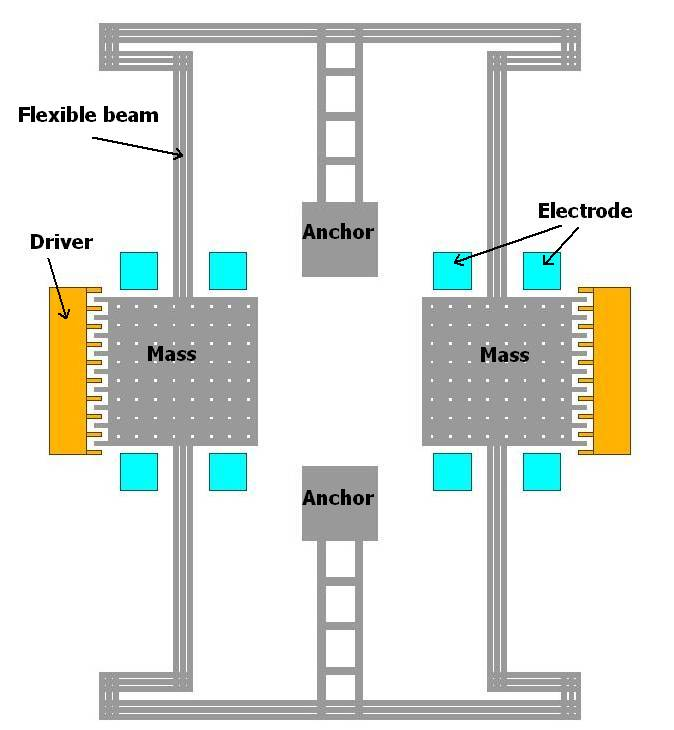
\includegraphics[width=.7\textwidth]{tuning-fork-gyro}
\end{center}
\caption{Giroscópio diapasão (Cortesia de Zhili Hao, Old Dominion University)}\label{fig.tuning-gyro-image}
\end{figure}

A teoria de funcionamento do giroscópio do garfo oscilante é mostrada na Fig.~\ref{fig.tuning-gyro}. As massas (quadrados cinza) são forçadas a vibrar na mesma frequência como os dois dentes de um garfo oscilante. Elas vibram em sentidos diferentes, ou seja, ou se aproximam uma da outra (setas com pontos azuis) ou se afastam uma da outra (setas vermelhas tracejadas). O componente gira em torno de um eixo perpendicular a seu centro (o círculo com uma cruz denota o eixo de rotação que é perpendicular ao plano do papel). A força de Coriolis é uma força cuja direção e sentido são dados pelo produto vetorial do eixo de rotação e do eixo de movimento da massa, e cuja magnitude é proporcional à velocidade linear da massa e à velocidade angular do giroscópio. Como as massas estão se movendo em sentidos opostos, as forças resultantes serão iguais, com mesma direção, mas em sentidos opostos (setas sólidas). As massas se aproximam ou retrocedem dos eletrodos (pequenos retângulos) e a mudança na capacitância pode ser medida por um circuito.

\begin{figure}
\begin{center}
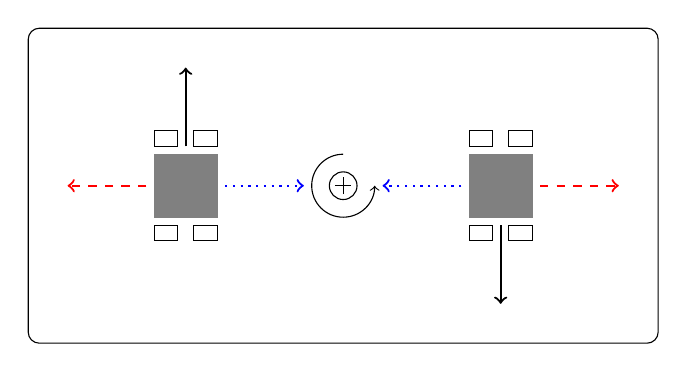
\begin{tikzpicture}
\draw[thin,rounded corners] (-4,-2) -- (4,-2) -- (4,2) -- (-4,2) -- cycle;
\draw[fill,gray] (-24mm,-4mm) rectangle +(8mm,8mm);
\draw[->,thick,dotted,blue] (-15mm,0mm) -- (-5mm,0mm);
\draw[->,thick,dashed,red] (-25mm,0mm) -- (-35mm,0mm);
\draw[->,thick] (-2,5mm) -- (-2,15mm);
\draw[fill,gray] (16mm,-4mm) rectangle +(8mm,8mm);
\draw[->,thick,dotted,blue] (15mm,0mm) -- (5mm,0mm);
\draw[->,thick,dashed,red] (25mm,0mm) -- (35mm,0mm);
\draw[->,thick] (2,-5mm) -- (2,-15mm);
\draw (0,0) circle[radius=5pt];
\draw (-3pt,0) -- (3pt,0);
\draw (0,-3pt) -- (0,3pt);
\draw[<-] (4mm,0) arc [start angle=0, end angle=-270, radius=4mm];
\foreach \x/\y in {-24/5,-19/5,16/5,21/5,-24/-7,-19/-7,16/-7,21/-7} {
  \draw (\x mm, \y mm) rectangle +(3mm,2mm);
}
\end{tikzpicture}
\end{center}
\caption{Física de um giroscópio diapasão (garfo oscilante): setas vermelhas tracejadas e setas azuis pontilhadas indicam a direção e sentido da vibração; setas negras sólidas indeiam a força de Coriolis}\label{fig.tuning-gyro}
\end{figure}

\subsection{Aplicações}

Um sistema de navegação inercial tem três acelerômetros e três giroscópios para que a pose do veículo possa ser computada em três dimensões. Isto é necessário para aeronaves robóticas e outros veículos robóticos. Os airbags utilizam um acelerômetro que detecta a desaceleração rápida na direção frente-lombar que ocorre quando um carro freia bruscamente. Isto causa uma expansão explosiva do airbag. É possível conceber mais aplicações para estes componentes em automóveis. Um acelerômetro na direção ascendente pode detectar se o carro caiu em um buraco. Um giroscópio medindo a rotação ao redor do eixo vertical pode detectar derrapagens, enquanto o giroscópio medindo a rotação ao redor do eixo dianteiro-traseiro pode detectar se o carro está capotando.

%%%%%%%%%%%%%%%%%%%%%%%%%%%%%%%%%%%%%%%%%%%%%%%%%%%%%%%%%%%

\section{Graus de Liberdade e Número de Atuadores}\label{s.dof}

O número de \emph{graus de liberdade (DoF)} de um sistema é a dimensionalidade das coordenadas necessárias para descrever uma pose de um objeto, como a de um robô móvel ou a pose do efetuador de um manipulador robótico.\footnote{Esta seção e as seguintes são mais avançadas e podem ser puladas durante uma primeira leitura. Além disso, alguns dos exemplos são de manipuladores robóticos descritos em Chap.~\ref{ch.kinematics}.} Por exemplo, um helicóptero tem seis DoF porque pode mover-se nas três dimensões espaciais e pode girar ao redor dos três eixos. Portanto, uma coordenada de seis dimensões $(x,y,z,\phi,\phi,\psi,\theta)$ é necessária para descrever sua pose\footnote{N. do T.: Lembre-se de que o termo "pose" refere-se à posição e à orientação do objeto.}.

\begin{quote}
\begin{center}
\textbf{Termos usados para descrever rotações}
\end{center}
Um helicóptero pode girar ao redor de todos os três eixos. As rotações são chamadas: (a) arfagem (\emph{pitch}): o nariz se move para cima e para baixo; (b) rolamento (\emph{roll}): o corpo gira ao redor de seu eixo longitudinal; (c) guinada (\emph{yaw}): o corpo gira à esquerda e à direita ao redor do eixo de seu rotor.
\end{quote}

O braço robótico de dois elos em Fig.~\ref{fig.two-link} tem apenas dois DoF porque seu efeito final se move em um plano e não gira; portanto, pode ser descrito por uma coordenada bidimensional $(x,y)$. Ao examinar novamente a Fig.~\ref{fig.pos-head}, você pode ver que um robô móvel movendo-se em uma superfície plana tem três DoF porque sua pose é definida por uma coordenada tridimensional $(x,y,\theta)$. Um trem tem apenas um DoF, uma vez que é obrigado pelos trilhos a se mover para frente (ou ocasionalmente para trás) ao longo da linha. É preciso apenas uma coordenada $(x)$, a distância do trem a uma origem arbitrária da via, para especificar a pose do trem.

\begin{figure}
\begin{center}
% Forward kinematics
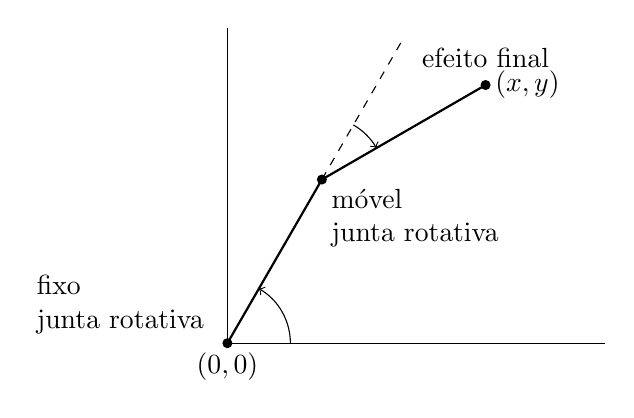
\begin{tikzpicture}[scale=.8,align=left]
\draw (0,0) coordinate (origin) -- (6,0);
\draw (origin) -- (0,5);
\draw[thick] (origin) -- ++(60:3) coordinate (prime) -- ++(30:3) coordinate (point);
\path (origin) -- ++(60:3) -- ++(30:1) coordinate (angle);
\draw[dashed] (60:3) -- ++(60:2.6);
\draw[->] (1,0) arc (0:60:1);
\draw[<-] (angle) arc (30:60:1);
\draw[fill] (origin) circle [radius=2pt] node[below] {$(0,0)$};
\draw[fill] (prime) circle [radius=2pt];
\draw[fill] (point) circle [radius=2pt] node[right] {$(x,y)$};
\node[above,yshift=1mm] at (point) {\p{efeito final}};
\node[above left,xshift=-5pt] at (origin) {\p{fixo}\\\p{junta rotativa}};
\node[below right] at (prime) {\p{móvel}\\\p{junta rotativa}};
\end{tikzpicture}
\end{center}
\caption{Um braço robótico de dois elos com dois DoF}\label{fig.two-link}
\end{figure}

Precisamos de mais informações do que os graus de liberdade para descrever o movimento robótico. Considere um veículo como um carro, uma bicicleta ou uma cadeira de escritório. Embora três coordenadas $(x,y,\theta)$ sejam necessárias para descrever sua pose, não podemos necessariamente mover o veículo diretamente de uma pose para outra. Uma cadeira de escritório pode ser movida \emph{diretamente} para qualquer ponto do plano e orientada em qualquer direção. Um carro ou uma bicicleta a $(2,0,0^\circ)$ (orientada na direção do eixo positivo $x$) não pode ser movida diretamente para cima do eixo $y$ para a posição $(2,2,0^\circ)$. Uma manobra mais complexa é necessária.

Precisamos saber o número de seus \emph{atuadores} (geralmente motores) e sua configuração. Um robô móvel de acionamento diferencial tem dois atuadores, um para cada roda, embora o próprio robô tenha três DoF. Os motores movem o robô ao longo de um eixo para frente e para trás, mas aplicando uma potência diferente a cada motor podemos mudar a orientação do robô. O braço de dois elos na Fig.~\ref{fig.two-link} tem dois motores, um em cada junta rotativa, portanto o número de atuadores é igual ao número de DoF. Finalmente, um trem tem apenas um atuador, o motor que o move para frente ou para trás em seu único DoF\footnote{N. do T.: Ainda que um trem tenha vários motores, todos atuam em paralelo e resultam num mesmo movimento. Para efeitos de análise, tudo se passe como se existisse apenas um atuador.}.

\begin{framed}
\act{Robô que só pode girar}{rotate-only}
\begin{itemize}
\item A figura~\ref{fig.rot-dof} mostra um robô de acionamento diferencial com uma haste fixa através de seu centro de rotação. A haste impede que o robô mude de posição, permitindo que ele só gire em torno de seu eixo vertical. Caracterize esta configuração: o número de atuadores e o número de DoF.
\item Que tipos de tarefas este robô poderia realizar? Quais são as vantagens e desvantagens desta configuração?
\end{itemize}
\end{framed}

\begin{figure}
\begin{center}
\begin{tikzpicture}[scale=1.3]
\begin{scope}[rotate=30]
\coordinate (origin) at (0,0);
\pic[scale=1.6,rotate=30] at (origin) {robot};
\fill[gray!80] (origin) circle [radius=2mm];
\draw[raxis] (0,0) -- (-8pt,0);
\draw[raxis] (0,0) -- (8pt,0);
\draw[->,thick] ($(origin)+(-5pt,10pt)$) arc (130:-10:9pt);
\end{scope}
\draw[raxis] (0,0) -- (120:15mm);
\draw[raxis] (0,0) -- (300:15mm);
\end{tikzpicture}
\end{center}
\caption{Um robô que só pode girar em torno de um eixo (ponto cinza)}\label{fig.rot-dof}
\end{figure}

\section{O Número Relativo de Atuadores e Graus de Liberdade (DoF)}\label{s.num-actuators}

Vamos analisar os sistemas onde:
\begin{itemize}
\item O número de atuadores é igual ao número de DoF;
\item O número de atuadores é menor do que o número de DoF;
\item O número de atuadores é maior do que o número de DoF.
\end{itemize}

\subsubsection*{O Número de Atuadores é Igual ao Número de DoF}

Um trem tem um atuador (seu motor) que move o trem ao longo de seu único DoF. O braço robótico de dois elos da Fig.~\ref{fig.two-link} tem dois atuadores e dois DoF. Uma garra robótica pode ser construída com três motores que giram a garra em cada uma das três orientações (rolamento, arfagem, guinada). A vantagem de ter um número igual de atuadores e DoF é que o sistema é relativamente fácil de controlar: cada atuador é comandado individualmente para mover o robô para a posição desejada no DoF que ele controla.

\subsubsection*{O Número de Atuadores é Menor do que o Número de DoF}

Os robôs móveis geralmente têm menos atuadores do que o DoF. Um robô com acionamento diferencial e um carro têm apenas dois atuadores, mas podem alcançar todas as poses possíveis num plano. Ter menos atuadores torna o sistema menos caro, mas os problemas de planejamento e controle de movimento são muito mais difíceis. O estacionamento paralelo de um carro é notório por sua dificuldade: são necessárias duas rotações e uma translação para realizar um simples movimento lateral (Figs.~\ref{fig.parallel-diff}--\ref{fig.parallel-car}).

Um exemplo extremo é um balão de ar quente que tem apenas um único atuador (um aquecedor) que injeta mais ou menos ar quente no balão e assim controla sua altitude. Entretanto, os ventos podem fazer com que o balão se mova em qualquer uma das três direções espaciais e até mesmo girar (pelo menos parcialmente) em três orientações, de modo que o operador do balão nunca pode controlar com precisão a sua pose. Portanto, um balão de ar quente difere de um elevador: ambos têm um único atuador, mas o elevador é obrigado por seu eixo a se mover em apenas um DoF.

Para outro exemplo da complexa relação entre o número de DoF e o número de atuadores, o leitor é convidado a estudar o controle de voo em helicópteros. Os helicópteros são altamente manobráveis (ainda mais que os aviões, que não podem voar para trás), mas um piloto controla o voo do helicóptero usando apenas três atuadores:
\begin{itemize}
\item O \bold{cíclico} controla o passo do eixo do rotor principal, que determina se o helicóptero se move para frente, para trás ou para ambos os lados.
\item O \bold{coletivo} controla o passo das lâminas do rotor principal, que determina se o helicóptero se move para cima ou para baixo.
\item Os \bold{pedais} controlam a velocidade do rotor de cauda que determina a direção em que o nariz do helicóptero aponta.
\end{itemize}

\subsubsection*{O Número de Atuadores é Maior do que o Número de DoF}

Não parece ser uma boa ideia ter mais atuadores do que o DoF, mas na prática tais configurações são muitas vezes úteis. Os sistemas na Figs.~\ref{fig.hi-act-low-dof-1}--\ref{fig.hi-act-low-dof-2} têm mais atuadores do que DoF. O braço manipulador robótico na Figs.~\ref{fig.hi-act-low-dof-1} tem quatro elos girando no plano com atuadores (motores) \p{a1}, \p{a2}, \p{a3}, \p{a4} em cada uma das juntas. Assumimos que o efetuador seja fixado ao elo a partir de \p{a4} e não possa girar, portanto sua pose é definida por sua posição $(x,y)$ e uma orientação fixa. Logo, embora o braço tenha quatro atuadores, ele possui apenas dois DoF porque pode mover o efetuador apenas no plano $(x,y)$ (horizontal e verticalmente).

O robô móvel com um braço (Fig.~\ref{fig.hi-act-low-dof-2}) tem três atuadores: um motor que move o robô para frente e para trás, e motores para cada uma das duas juntas rotativas do manipulador. Entretanto, o sistema tem apenas dois DoF já que a pose de seu efetuador é definida por uma coordenada bidimensional de $(x,y)$. Sistemas com mais atuadores que DoF são chamados de \emph{sistemas redundantes}.

\begin{figure}
\begin{minipage}{.45\textwidth}
\begin{tikzpicture}[scale=1.2]
\coordinate (j1) at (1,0);
\fill[gray!50] (0,-2mm) rectangle +(4,-2mm);
\draw[very thick] (j1) -- +(0,-2mm);
\draw[thick] (j1) node[above right,xshift=5pt] {\p{a1}} -- ++(120:10mm) coordinate (j2) node[left,xshift=-2pt,yshift=-2pt] {\p{a2}} -- ++(30:15mm) coordinate (j3) node[above left,xshift=-4pt,yshift=-2pt] {\p{a3}} -- ++(10:12mm) coordinate (j4) node[right,xshift=2pt,yshift=-2pt] {\p{a4}} -- ++(80:8mm) coordinate (ee) node[left,xshift=-2pt] {\p{efetuador}};
\draw[->] ($(j1)+(-7pt,2pt)$) arc (180:0:6pt);
\draw[->] ($(j2)+(-5pt,4pt)$) arc (140:-40:6pt);
\draw[->] ($(j3)+(-5pt,2pt)$) arc (160:-60:6pt);
\draw[->] ($(j4)+(-6pt,2pt)$) arc (180:0:6pt);
\fill (j1) circle [radius=2pt];
\fill (j2) circle [radius=2pt];
\fill (j3) circle [radius=2pt];
\fill (j4) circle [radius=2pt];
\fill (ee) circle [radius=2pt];
\end{tikzpicture}
\caption{Braço robótico: dois DoF e quatro atuadores}\label{fig.hi-act-low-dof-1}
\end{minipage}
\hspace{\fill}
\begin{minipage}{.45\textwidth}
\begin{tikzpicture}[scale=1.2]
\fill[gray!50] (0,-3mm) rectangle +(4,-2mm);
\draw[rounded corners] (4mm,0) rectangle +(3,1);
\draw[fill=white] (11mm,0) circle [radius=3mm];
\draw[fill=white] (29mm,0) circle [radius=3mm];
\draw[raxis] (11mm,0) -- +(-2mm,0);
\draw[raxis] (11mm,0) -- +(2mm,0);
\draw[raxis] (11mm,0) -- +(0,2mm);
\draw[raxis] (11mm,0) -- +(0,-2mm);
\draw[raxis] (29mm,0) -- +(-2mm,0);
\draw[raxis] (29mm,0) -- +(2mm,0);
\draw[raxis] (29mm,0) -- +(0,2mm);
\draw[raxis] (29mm,0) -- +(0,-2mm);
\draw (17mm,1) coordinate (j1) node[above right] {\p{a1}} -- ++(130:10mm) coordinate (j2) node[left,xshift=-2pt] {\p{a2}} -- ++(60:10mm) coordinate (ee) node[right,xshift=2pt] {\p{efetuador}};
\draw[->] ($(j1)+(0pt,-5pt)$) arc (-90:-270:6pt);
\draw[->] ($(j2)+(-3pt,6pt)$) arc (120:-100:6pt);
\fill (j1) circle [radius=2pt];
\fill (j2) circle [radius=2pt];
\fill (ee) circle [radius=2pt];
\end{tikzpicture}
\caption{Robô móvel e manipulador: dois DoF e três atuadores}\label{fig.hi-act-low-dof-2}
\end{minipage}
\end{figure}

%\begin{figure}
%\subfigures
%\leftfigure{
%\begin{tikzpicture}[scale=1.2]
%\coordinate (j1) at (1,0);
%\fill[gray!50] (0,-2mm) rectangle +(4,-2mm);
%\draw[very thick] (j1) -- +(0,-2mm);
%\draw[thick] (j1) node[above right,xshift=5pt] {\p{a1}} -- ++(120:10mm) coordinate (j2) node[left,xshift=-2pt,yshift=-2pt] {\p{a2}} -- ++(30:15mm) coordinate (j3) node[above left,xshift=-4pt,yshift=-2pt] {\p{a3}} -- ++(10:12mm) coordinate (j4) node[right,xshift=2pt,yshift=-2pt] {\p{a4}} -- ++(80:8mm) coordinate (ee) node[left,xshift=-2pt] {\p{end effector}};
%\draw[->] ($(j1)+(-7pt,2pt)$) arc (180:0:6pt);
%\draw[->] ($(j2)+(-5pt,4pt)$) arc (140:-40:6pt);
%\draw[->] ($(j3)+(-5pt,2pt)$) arc (160:-60:6pt);
%\draw[->] ($(j4)+(-6pt,2pt)$) arc (180:0:6pt);
%\fill (j1) circle [radius=2pt];
%\fill (j2) circle [radius=2pt];
%\fill (j3) circle [radius=2pt];
%\fill (j4) circle [radius=2pt];
%\fill (ee) circle [radius=2pt];
%\end{tikzpicture}
%}
%\hspace{\fill}
%\rightfigure{
%\begin{tikzpicture}[scale=1.2]
%\fill[gray!50] (0,-3mm) rectangle +(4,-2mm);
%\draw[rounded corners] (4mm,0) rectangle +(3,1);
%\draw[fill=white] (11mm,0) circle [radius=3mm];
%\draw[fill=white] (29mm,0) circle [radius=3mm];
%\draw[raxis] (11mm,0) -- +(-2mm,0);
%\draw[raxis] (11mm,0) -- +(2mm,0);
%\draw[raxis] (11mm,0) -- +(0,2mm);
%\draw[raxis] (11mm,0) -- +(0,-2mm);
%\draw[raxis] (29mm,0) -- +(-2mm,0);
%\draw[raxis] (29mm,0) -- +(2mm,0);
%\draw[raxis] (29mm,0) -- +(0,2mm);
%\draw[raxis] (29mm,0) -- +(0,-2mm);
%\draw (17mm,1) coordinate (j1) node[above right] {\p{a1}} -- ++(130:10mm) coordinate (j2) node[left,xshift=-2pt] {\p{a2}} -- ++(60:10mm) coordinate (ee) node[right,xshift=2pt] {\p{end effector}};
%\draw[->] ($(j1)+(0pt,-5pt)$) arc (-90:-270:6pt);
%\draw[->] ($(j2)+(-3pt,6pt)$) arc (120:-100:6pt);
%\fill (j1) circle [radius=2pt];
%\fill (j2) circle [radius=2pt];
%\fill (ee) circle [radius=2pt];
%\end{tikzpicture}
%}
%\leftcaption{Robot arm: two DOF and four actuators}\label{fig.hi-act-low-dof-1}
%\rightcaption{Mobile robot and arm: two DOF and three actuators}\label{fig.hi-act-low-dof-2}
%\end{figure}

Se possível, os engenheiros evitam usar mais de um atuador agindo sobre um mesmo DoF porque isso aumenta a complexidade e o custo de um sistema. A cinemática inversa (Sect.~\ref{s.inverse-kinematics}) de um sistema redundante resulta em um número infinito de soluções que complicam sua operação. Para o robô móvel com manipulador (Fig.~\ref{fig.hi-act-low-dof-2}), há um número infinito de posições da base e do braço que levam o efetuador a uma posição específica alcançável.

Há situações em que é necessário um sistema redundante porque a tarefa não poderia ser realizada com menos atuadores. A Figura~\ref{fig.redundant1} mostra como o braço robótico de quatro elos da Fig.~\ref{fig.hi-act-low-dof-1} pode mover o efetor final para uma posição bloqueada por um obstáculo e, portanto, inalcançável por um braço de dois elos (Fig.~\ref{fig.redundant2}), mesmo que em ambas as configurações o comprimento total dos elos seja igual.

\begin{figure}
\begin{minipage}{.45\textwidth}
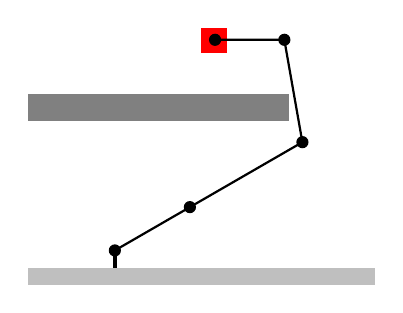
\begin{tikzpicture}[scale=1.1]
\coordinate (j1) at (1,0);
\fill[gray!50] (0,-2mm) rectangle +(4,-2mm);
\draw[very thick] (j1) -- +(0,-2mm);
\draw[fill,gray] (0,15mm) rectangle +(30mm,3mm);
\draw[red,fill] (57pt,65pt) rectangle +(8pt,8pt);
%\draw (0,0) -- (1,0) coordinate (j1)-- (4,0);
\draw[thick] (j1) -- ++(30:10mm) coordinate (j2) -- ++(30:15mm) coordinate (j3) -- ++(100:12mm) coordinate (j4) -- ++(180:8mm) coordinate (ee);
\fill (j1) circle [radius=2pt];
\fill (j2) circle [radius=2pt];
\fill (j3) circle [radius=2pt];
\fill (j4) circle [radius=2pt];
\fill (ee) circle [radius=2pt];
\end{tikzpicture}
\caption{Braço com quatro atuadores pode alcançar uma posição atrás de um obstáculo}\label{fig.redundant1}
\end{minipage}
\hspace{\fill}
\begin{minipage}{.45\textwidth}
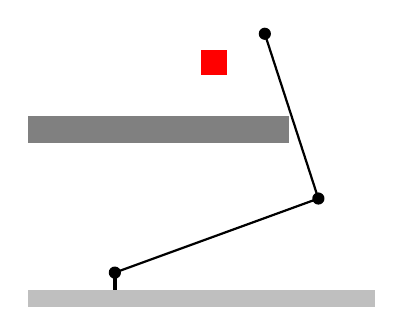
\begin{tikzpicture}[scale=1.1]
\coordinate (j1) at (1,0);
\fill[gray!50] (0,-2mm) rectangle +(4,-2mm);
\draw[very thick] (j1) -- +(0,-2mm);
\draw[fill,gray] (0,15mm) rectangle +(30mm,3mm);
\draw[red,fill] (57pt,65pt) rectangle +(8pt,8pt);
%\draw (0,0) -- (1,0) coordinate (j1)-- (4,0);
\draw[thick] (j1) -- ++(20:25mm) coordinate (j2) -- ++(108:20mm) coordinate (ee);
\fill (j1) circle [radius=2pt];
\fill (j2) circle [radius=2pt];
\fill (ee) circle [radius=2pt];
\end{tikzpicture}
\caption{Braço com dois atuadores é bloqueado por um obstáculo}\label{fig.redundant2}
\end{minipage}
\end{figure}


%\begin{figure}
%\subfigures
%\leftfigure{
%\begin{tikzpicture}[scale=1.1]
%\coordinate (j1) at (1,0);
%\fill[gray!50] (0,-2mm) rectangle +(4,-2mm);
%\draw[very thick] (j1) -- +(0,-2mm);
%\draw[fill,gray] (0,15mm) rectangle +(30mm,3mm);
%\draw[red,fill] (57pt,65pt) rectangle +(8pt,8pt);
%%\draw (0,0) -- (1,0) coordinate (j1)-- (4,0);
%\draw[thick] (j1) -- ++(30:10mm) coordinate (j2) -- ++(30:15mm) coordinate (j3) -- ++(100:12mm) coordinate (j4) -- ++(180:8mm) coordinate (ee);
%\fill (j1) circle [radius=2pt];
%\fill (j2) circle [radius=2pt];
%\fill (j3) circle [radius=2pt];
%\fill (j4) circle [radius=2pt];
%\fill (ee) circle [radius=2pt];
%\end{tikzpicture}
%}
%\hspace{\fill}
%\rightfigure{
%\begin{tikzpicture}[scale=1.1]
%\coordinate (j1) at (1,0);
%\fill[gray!50] (0,-2mm) rectangle +(4,-2mm);
%\draw[very thick] (j1) -- +(0,-2mm);
%\draw[fill,gray] (0,15mm) rectangle +(30mm,3mm);
%\draw[red,fill] (57pt,65pt) rectangle +(8pt,8pt);
%%\draw (0,0) -- (1,0) coordinate (j1)-- (4,0);
%\draw[thick] (j1) -- ++(20:25mm) coordinate (j2) -- ++(108:20mm) coordinate (ee);
%\fill (j1) circle [radius=2pt];
%\fill (j2) circle [radius=2pt];
%\fill (ee) circle [radius=2pt];
%\end{tikzpicture}
%}
%\leftcaption{Arm with four actuators can reach a hidden position}\label{fig.redundant1}
%\rightcaption{Arm with two actuators is blocked by an obstacle}\label{fig.redundant2}
%\end{figure}

Uma vantagem importante dos sistemas redundantes surge de atuadores com características diferentes. O robô móvel na Fig.~\ref{fig.hi-act-low-dof-2} pode se aproximar rapidamente do alvo, embora sua posição final possa não ser precisa por causa de erros como terreno irregular. Uma vez que o robô móvel pare, os motores nas juntas que não têm de lidar com o terreno podem ser posicionados com precisão. Embora o posicionamento seja preciso, estas juntas sozinhas não podem proporcionar o mesmo alcance da base móvel.


\subsubsection*{Um Exemplo de um Sistema com Mais Atuadores do que DoF}

A figura~\ref{fig.act-dof} (vista superior e lateral) mostra uma configuração com \emph{dois atuadores e um DoF}. O sistema modela um guindaste robótico que move um objeto pesado para uma posição vertical específica. A figura ~\ref{fig.crane} mostra um guindaste construído a partir de um robô Thymio e componentes de \lego.\footnote{O guincho está à direita do robô e não à esquerda como na figura~\ref{fig.act-dof}.}

\begin{figure}
\begin{center}
\begin{tikzpicture}[align=left]
%
% Top view
%
\begin{scope}[scale=2.3,xshift=25mm]
% Table
\draw[fill,gray!20] (-34mm,-26mm) rectangle +(40mm,30mm);
% Robot
\draw (0,0) to [rounded corners] (-20mm,0) to [rounded corners, bend right=45] (-20mm,-18mm) to (0,-18mm) to cycle;
% Drive wheels
\fill (-11mm,0) rectangle +(8mm, 2mm);
\fill (-11mm,-18mm) rectangle +(8mm, -2mm);
\node at (-12mm,-8mm) {\p{rodas de tração}};
\draw[->] (-8mm,-6mm) -- +(0,14pt);
\draw[->] (-8mm,-10mm) -- +(0,-20pt);
% Road wheels
\fill[gray!70] (-3mm,0) rectangle +(10mm, 2mm) node[above left,black,xshift=-38pt,yshift=13pt] {\p{roda de deslocamento}};
\draw[->] (1mm,5mm) -- +(0,-8pt);
\fill[gray!70] (-3mm,-23mm) rectangle +(10mm, -2mm);
\draw[fill,cyan] (2mm,0) rectangle +(2pt,-23mm);
\draw[fill,cyan] (2mm,-9mm) rectangle +(-4mm,2pt);
\draw[raxis] (2.4mm,-25.6mm) -- +(0,29mm);
% Winch
\fill[red] (-9mm,-20mm) rectangle +(4mm, -2mm) node[below left,black,xshift=-18pt,yshift=-7pt] {\p{guincho}};
\draw[->] (-8mm,-25mm) -- +(0,8pt);
\draw[raxis] (-7mm,-24mm) -- +(0,27mm);
% Weight
\fill[red] (-41.1mm,-22mm) rectangle +(1.5mm,2mm);
% Bearing
\fill[gray!70] (-40mm,-22.8mm) rectangle +(2mm,4mm) node[above,xshift=-4mm,black,yshift=6pt] {\p{rolamento e}\\\p{peso}};
\draw[raxis] (-39mm,-23.8mm) -- +(0,6mm);
% Cable
\draw[thick,red] (-9mm,-21mm) -- ++(-32mm,0);
\end{scope}
%
% Side view
%
\begin{scope}[yshift=-10.5cm]
% Table
\draw[fill,gray!20] (-2,-23.5mm) rectangle +(9.5,2mm);
\draw[fill,gray!20] (-1,-23.5mm) rectangle +(4mm,-15mm);
\draw[fill,gray!20] (5,-23.5mm) rectangle +(4mm,-15mm);
% Big wheel
\draw[fill,gray!70] (62mm,-9mm) circle[radius=1.25] node[left,black,xshift=-34pt,yshift=-8pt] {\p{roda de deslocamento}};
% Attachment
\draw[fill,cyan] (62mm,-9mm) circle[radius=4pt];
\draw[fill,cyan] (61.5mm,-9mm) rectangle +(3pt,20.5mm);
\draw[fill,cyan] (62.5mm,11mm) rectangle +(-5mm,3pt);
% Axis intersection of big wheel
\draw[raxis] (62mm,-9mm) -- +(24pt,0);
\draw[raxis] (62mm,-9mm) -- +(-24pt,0);
\draw[raxis] (62mm,-9mm) -- +(0,24pt);
\draw[raxis] (62mm,-9mm) -- +(0,-24pt);
% Robot
\draw[rounded corners,fill=white] (.2,0) -- (.2,2) -- (5.9, 2) -- (5.9,0) -- cycle;
% Wheel
\draw[fill,black] (4.3,9pt) circle[radius=1] node[left,black,xshift=-24pt,yshift=23pt] {\p{roda de tração}};
% Winch
\draw[fill,red]  (4.3,9pt) circle[radius=.5] node[above right,black,xshift=5pt,yshift=28pt] {\p{guincho}};
\draw[->] (5,39pt) -- +(-16pt,-24pt);
\draw[raxis] (4.3,9pt) -- +(14pt,0);
\draw[raxis] (4.3,9pt) -- +(-14pt,0);
\draw[raxis] (4.3,9pt) -- +(0,14pt);
\draw[raxis] (4.3,9pt) -- +(0,-14pt);
% Support
\draw[fill,gray!70] (.9,0) rectangle +(.8,-17.5mm);
\draw[fill,gray!70] (.9,-17.5mm) arc(180:360:4mm);
% Bearing
\draw[red,fill=gray!70] (-85pt,13pt) circle[radius=10pt] node[above,black,yshift=4mm] {\p{rolamento}};
\draw[thick,red] (4.3,23pt) -- (-85pt,23pt);
\draw[raxis] (-85pt,13pt) -- +(8pt,0);
\draw[raxis] (-85pt,13pt) -- +(-8pt,0);
\draw[raxis] (-85pt,13pt) -- +(0,8pt);
\draw[raxis] (-85pt,13pt) -- +(0,-8pt);
% Weight
\draw[thick,red] (-95pt,13pt) -- ++(0,-100pt);
\draw[fill,red] (-101pt,-95pt) rectangle +(12pt,12pt) node[right,black] {\p{peso}};
\end{scope}
\end{tikzpicture}
\caption{Guindaste robótico construído a partir de um robô móvel e um guincho (vista superior acima, vista lateral abaixo); na vista lateral a roda esquerda não é mostrada}\label{fig.act-dof}
\end{center}
\end{figure}

\begin{figure}
\begin{center}
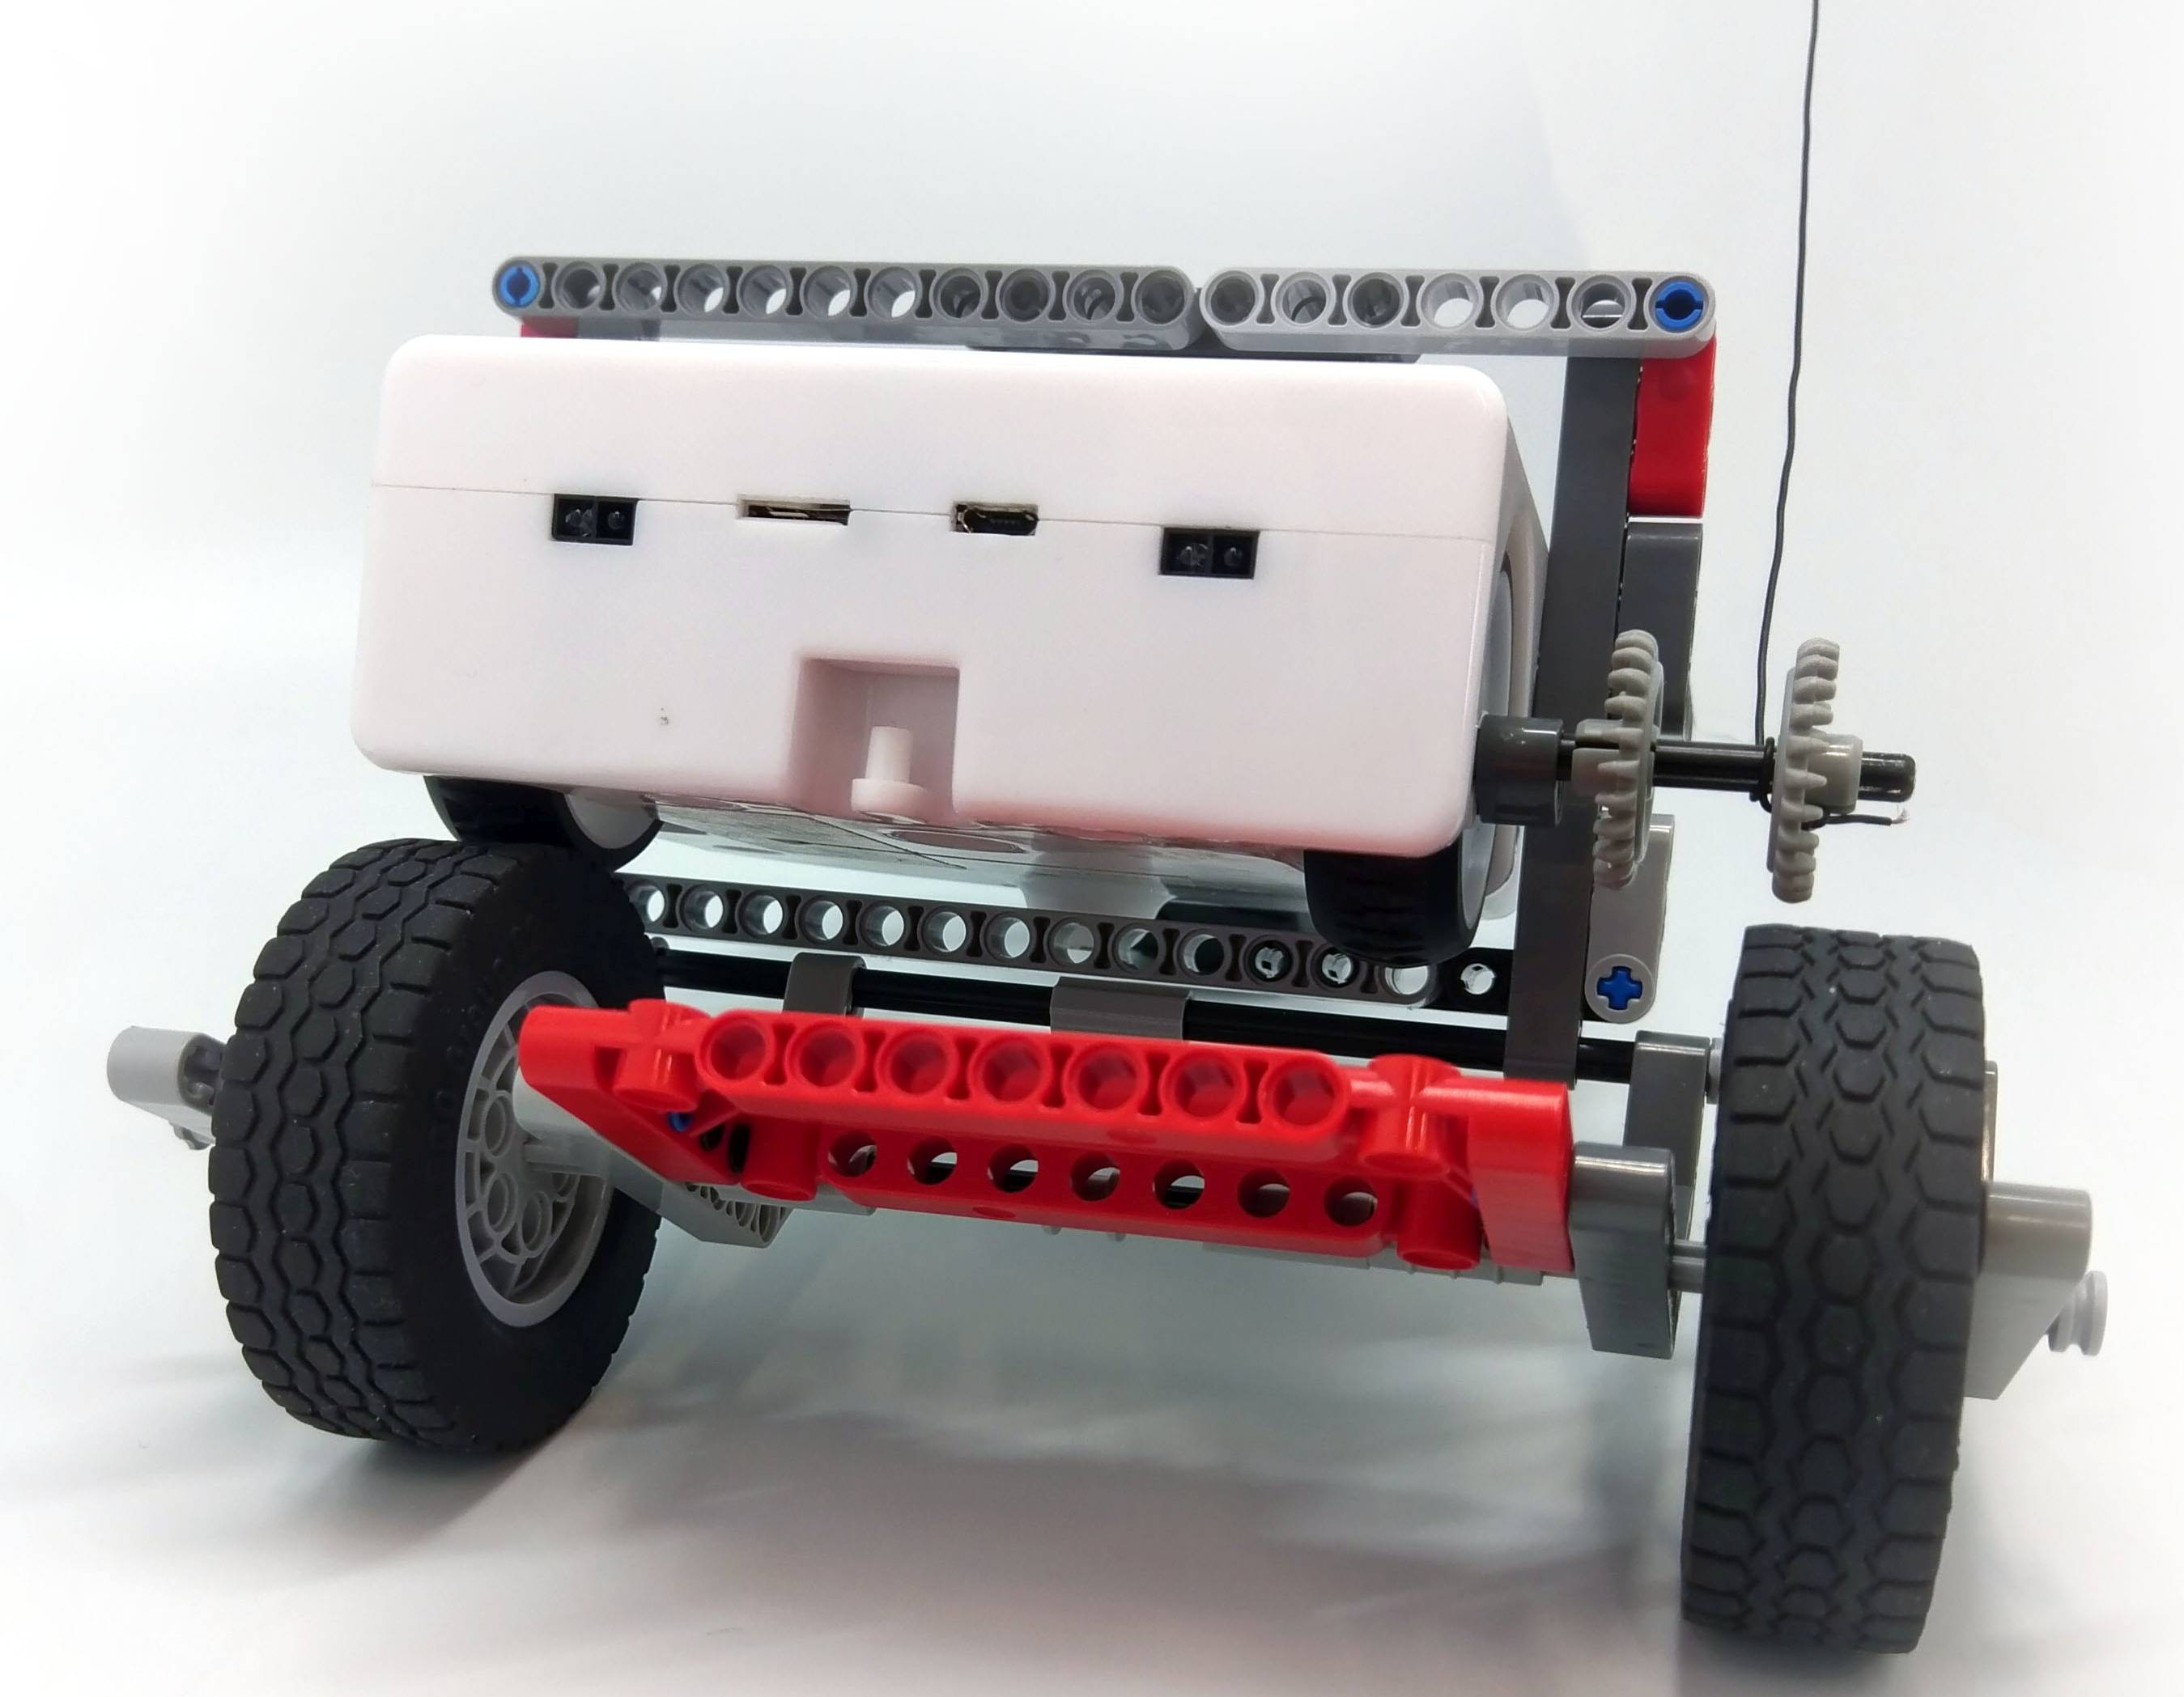
\includegraphics[width=.8\textwidth]{robotic-crane.jpg}
\caption{Guindaste robótico construído a partir de um robô Thymio e componentes \lego}\label{fig.crane}
\end{center}
\end{figure}

O sistema é construído a partir de um robô móvel com tração diferencial, mas as rodas não são usadas diretamente para controlar o movimento do sistema. Ao invés disso, cada roda é um atuador independente. (Lembre-se que a potência de cada roda de um robô com acionamento diferencial pode ser ajustada independentemente para qualquer valor em uma faixa como $-100$ a $100$).

O robô está virado para a esquerda. A roda acionada à direita na Fig.~\ref{fig.act-dof} (o retângulo preto no topo da vista superior e oculto atrás do robô na vista lateral) controla um par de rodas (cinzas) que movem o robô rapidamente para frente e para trás. Por sua vez, isto faz com que o cabo mova o peso rapidamente para cima e para baixo.

As rodas de deslocamento são montadas em uma estrutura (em azul) que é fixada ao corpo do robô. Há várias opções para transferir a potência da roda de tração direita para as rodas de deslocamento: atrito, roldanas e correias e engrenagens. Cada opção tem suas próprias vantagens e desvantagens, e todas as três são usadas em carros: a embreagem usa fricção, correias são usadas para o sincronismo e para operar componentes auxiliares como bombas d'água, e engrenagens são usadas na transmissão para controlar o torque aplicado a cada roda.

A roda de tração à esquerda (o retângulo preto na parte inferior da vista superior e na frente da vista lateral) controla um guincho (vermelho) que enrola ou desenrola um cabo preso ao peso que se move para cima ou para baixo sobre um rolamento fixo. O guincho tem um diâmetro muito menor do que o diâmetro das rodas acionadas, de modo que ele pode mover o peso em pequenos incrementos à medida que a roda acionada à esquerda gira. O objetivo do projeto é ser capaz de realizar o posicionamento preciso do peso mesmo que o guincho mova o cabo a uma velocidade muito mais lenta do que o corpo do robô.

Há duas atividades para esta seção. Esta atividade é para leitores que possuem boas habilidades de construção e um kit de robótica apropriado. A segunda atividade sugere formas alternativas de demonstrar o conceito de dois atuadores em um DoF.

\begin{framed}
\act{Guindaste robótico}{act-dof}
\begin{itemize}
\item Construa o guindaste robótico mostrado na Fig.~\ref{fig.act-dof}. Explique sua escolha de mecanismo para conectar a roda de tração às rodas de deslocamento.
\item Escreva um programa que, dada a posição atual do peso e uma posição desejada, mova o peso para a posição desejada. Alternativamente, envie comandos para os motores usando um dispositivo de controle remoto ou um computador conectado ao robô.
\item Experimente as velocidades relativas de rotação das rodas acionadas à esquerda e à direita que controlam as rodas e o guincho, respectivamente. Você deve mover os dois atuadores separadamente ou simultaneamente?
\end{itemize}
\end{framed}

\begin{framed}
\act{Guindaste robótico (alternativas)}{act-dof-alt}
\begin{itemize}
\item Escreva um programa que faz com que um robô móvel se mova para frente e para trás. Coloque um pedaço de fita preta relativamente longe da posição inicial do robô. O objetivo é fazer com que o robô pare o mais próximo possível do início da fita adesiva \emph{sem} verificação contínua do sensor. 
\item O programa tem três modos de operação. (1) O robô se move rapidamente, verificando seu sensor ocasionalmente e parando quando detecta a fita adesiva. (2) Como em (1), mas o robô move-se lentamente, verificando seu sensor com relativa frequência. (3) Como em (1), mas quando a fita é detectada, o robô se move para trás usando a velocidade e o período de amostragem como em (2).
\item Execute o programa e compare os resultados dos três modos: o tempo até que o robô pare e o erro entre a posição final do robô e o início da fita adesiva.
\item Como alternativa, execute o programa com os três modos em um computador e experimente com os parâmetros de movimento e os períodos de amostragem. Você precisará escolher um modelo para o movimento: velocidade constante, aceleração constante, ou (mais realista) aceleração seguida de velocidade constante e finalmente desaceleração quando a fita for detectada.
\end{itemize}
\end{framed}

%%%%%%%%%%%%%%%%%%%%%%%%%%%%%%%%%%%%%%%%%%%%%%%%%%%%%%%%%%%


\section{Movimento holonômico e não-holonômico}\label{s.holonomic}

A seção~\ref{s.dof} apresentou o conceito de graus de liberdade (DoF) e o papel do número de atuadores. Há outro conceito que liga os DoF e os atuadores no caso dos robôs móveis: os graus de mobilidade (em inglês, \emph{Degrees of Mobility - DoM}). Os graus de mobilidade $\delta_m$ correspondem ao número de graus de liberdade que podem ser \emph{acessados diretamente} pelos atuadores. Um robô móvel no plano tem no máximo três DoF ($(x,y)$ posição e orientação), portanto o maior número de graus de mobilidade de um robô móvel é $\delta_m = 3$.

Consideremos os DoM de vários veículos. Um trem tem um DoF porque só pode avançar ao longo dos trilhos, e tem um atuador, seu motor, que afeta diretamente este único grau de liberdade. Portanto, um trem tem um grau de mobilidade de $\delta_m = 1$, o que significa que o único DoF pode ser acessado diretamente pelo atuador.

Um robô com acionamento diferencial tem três DoF. Os dois atuadores são os dois motores que atuam sobre as rodas. Eles podem acessar diretamente dois DoF: (a) se as duas rodas giram na mesma velocidade, o robô se move para frente ou para trás; (b) se as rodas têm velocidades em direções opostas, o robô gira no lugar. Portanto, podemos acessar diretamente o DoF ao longo do eixo de translação para frente e o DoF da orientação, mas não podemos acessar diretamente o DoF do eixo lateral de translação (Fig.~\ref{fig.mobility-example1}). Um robô móvel de acionamento diferencial tem grau de mobilidade $\delta_m = 2 < 3 = \#\textrm{DoF}$.

\begin{figure}
\begin{minipage}{.45\textwidth}
\begin{tikzpicture}[align=left,scale=.9]
\coordinate (origin) at (0,0);
\pic[scale=2.2] at (origin) {robot};
\draw[<-,thick] ($(origin)+(4pt,20pt)$) arc (90:-90:20pt);
\draw[->,thick] ($(origin)+(10pt,0)$) -- +(95pt,0);
\node at (18mm,-9mm) {\p{acessível}\\\p{DOF}};
\draw[->] (18mm,-5mm) -- +(0,4mm);
\draw[->] (15mm,-5mm) -- +(-5mm,2mm);
\draw[->,thick,dashed] ($(origin)+(0,5pt)$) -- +(0,85pt);
\node at (18mm,26mm) {\p{não acessível}\\\p{DOF}};
\draw[->] (6mm,26mm) -- +(-5mm,0);
\end{tikzpicture}
\caption{DoF acessível e inacessível para um robô com acionamento diferencial}\label{fig.mobility-example1}
\end{minipage}
\hspace{\fill}
\begin{minipage}{.5\textwidth}
\begin{tikzpicture}[baseline=-20pt,align=left,scale=1.2]
\draw[rounded corners] (0,0) -- ++(4,0) -- ++(0,2) -- ++(-4,0) -- cycle;
\draw[rounded corners] (.5,.5) -- ++(1.5,0) -- ++(0,1) -- ++(-1.5,0) -- cycle;
\draw (.1,.1) -- (.5,.5);
\draw (.1,1.9) -- (.5,1.5);
\draw (2.4,.1) -- (2,.5);
\draw (2.4,1.9) -- (2,1.5);
\draw (2.5,.1) -- +(0,1.8);
\draw[<-,thick,dashed] (2.8,1.5) arc (90:-90:15pt);
\draw[->,thick] (3,1) -- +(45pt,0);
\draw[->,thick,dashed] (1.25,1) -- +(0,50pt);
\draw[fill,rotate around={30:(3.4,-.1)}] (3,-.2) rectangle +(.8,.2);
\draw[fill,rotate around={30:(3.4,2.1)}] (3,2) rectangle +(.8,.2);
\draw[fill] (.3,-2mm) rectangle +(.8,2mm);
\draw[fill] (.3,2) rectangle +(.8,2mm);
\node at (22mm,-4mm) {\p{acessível}\\\p{DOF}};
\draw[->] (26mm,-1mm) -- +(11mm,10mm);
\node at (26mm,25mm) {\p{não acessível}\\\p{DOF}};
\draw[->] (17mm,24mm) -- +(-4mm,0);
\draw[->] (25mm,23mm) -- +(4mm,-7mm);
\draw[raxis] (.7,-6mm) -- +(0,10mm);
\draw[raxis] (.7,16mm) -- +(0,10mm);
\draw[raxis] (3.4,-.1) -- +(120:4mm);
\draw[raxis] (3.4,-.1) -- +(300:4mm);
\draw[raxis] (3.4,2.1) -- +(120:4mm);
\draw[raxis] (3.4,2.1) -- +(300:4mm);
\end{tikzpicture}
\caption{DoF acessível e inacessível para um robô com direção Ackermann}\label{fig.mobility-example2}
\end{minipage}
\end{figure}


%\begin{figure}
%\subfigures
%\leftfigure
%{
%\begin{tikzpicture}[align=left,scale=.9]
%\coordinate (origin) at (0,0);
%\pic[scale=2.2] at (origin) {robot};
%\draw[<-,thick] ($(origin)+(4pt,20pt)$) arc (90:-90:20pt);
%\draw[->,thick] ($(origin)+(10pt,0)$) -- +(95pt,0);
%\node at (18mm,-9mm) {\p{accessible}\\\p{DOF}};
%\draw[->] (18mm,-5mm) -- +(0,4mm);
%\draw[->] (15mm,-5mm) -- +(-5mm,2mm);
%\draw[->,thick,dashed] ($(origin)+(0,5pt)$) -- +(0,85pt);
%\node at (18mm,26mm) {\p{non-accessible}\\\p{DOF}};
%\draw[->] (6mm,26mm) -- +(-5mm,0);
%\end{tikzpicture}
%}
%\hspace{\fill}
%\rightfigure
%{
%\begin{tikzpicture}[baseline=-20pt,align=left,scale=1.2]
%\draw[rounded corners] (0,0) -- ++(4,0) -- ++(0,2) -- ++(-4,0) -- cycle;
%\draw[rounded corners] (.5,.5) -- ++(1.5,0) -- ++(0,1) -- ++(-1.5,0) -- cycle;
%\draw (.1,.1) -- (.5,.5);
%\draw (.1,1.9) -- (.5,1.5);
%\draw (2.4,.1) -- (2,.5);
%\draw (2.4,1.9) -- (2,1.5);
%\draw (2.5,.1) -- +(0,1.8);
%\draw[<-,thick,dashed] (2.8,1.5) arc (90:-90:15pt);
%\draw[->,thick] (3,1) -- +(45pt,0);
%\draw[->,thick,dashed] (1.25,1) -- +(0,50pt);
%\draw[fill,rotate around={30:(3.4,-.1)}] (3,-.2) rectangle +(.8,.2);
%\draw[fill,rotate around={30:(3.4,2.1)}] (3,2) rectangle +(.8,.2);
%\draw[fill] (.3,-2mm) rectangle +(.8,2mm);
%\draw[fill] (.3,2) rectangle +(.8,2mm);
%\node at (22mm,-4mm) {\p{accessible}\\\p{DOF}};
%\draw[->] (26mm,-1mm) -- +(11mm,10mm);
%\node at (26mm,25mm) {\p{non-accessible}\\\p{DOF}};
%\draw[->] (17mm,24mm) -- +(-4mm,0);
%\draw[->] (25mm,23mm) -- +(4mm,-7mm);
%\draw[raxis] (.7,-6mm) -- +(0,10mm);
%\draw[raxis] (.7,16mm) -- +(0,10mm);
%\draw[raxis] (3.4,-.1) -- +(120:4mm);
%\draw[raxis] (3.4,-.1) -- +(300:4mm);
%\draw[raxis] (3.4,2.1) -- +(120:4mm);
%\draw[raxis] (3.4,2.1) -- +(300:4mm);
%\end{tikzpicture}
%}
%\leftcaption{Accessible and non-accesible DOF for a robot with differential drive}\label{fig.mobility-example1}
%\rightcaption{Accessible and non-accesible DOF for a robot with Ackermann steering}\label{fig.mobility-example2}
%\end{figure}

Um carro, assim como um robô com acionamento diferencial, tem apenas dois atuadores para três DoF: um atuador, o motor, dá acesso direto ao grau de liberdade ao longo do eixo longitudinal do carro, permitindo que ele se mova para frente e para trás. O outro atuador, o volante, \emph{não} dá acesso direto a nenhum DoF adicional, mas apenas orienta o primeiro DoF. O carro não pode girar ao redor do eixo vertical e não pode mover-se lateralmente (Fig.~\ref{fig.mobility-example2}). Portanto, um carro tem apenas um grau de mobilidade, $\delta_m = 1$. Intuitivamente, você pode ver o menor grau de mobilidade de um carro em comparação com um robô com tração diferencial, observando que o robô pode girar no lugar enquanto o carro não pode.

Por si só, uma roda padrão tem $\delta_m=2$: pode rolar para frente e para trás e pode girar ao redor do eixo vertical que passa pelo ponto de contato da roda com o solo. Uma roda não pode se mover lateralmente, o que desejável porque evita que o veículo derrape para fora da estrada durante uma curva. No carro, o grau de mobilidade é reduzido ainda mais para $\delta_m=1$, porque há dois pares de rodas, uma na frente e outra na traseira do carro. Esta configuração torna impossível que o carro gire em torno de seu eixo vertical, mesmo que as rodas individuais o possam fazer (geralmente apenas as rodas dianteiras). A limitação a $\delta_m=1$ dá estabilidade ao carro - não pode derrapar lateralmente e não pode girar - tornando fácil e seguro dirigir em altas velocidades. De fato, pode ocorrer um acidente quando a chuva ou a neve reduzem o atrito e o carro pode derrapar ou girar.

Um robô móvel autônomo pode se beneficiar se tiver um DoM maior $\delta_m = 3$. Para acessar diretamente o terceiro DoF, o robô precisa ser capaz de se mover lateralmente. Um método é ter o robô rolando sobre uma bola ou uma roda castor como uma cadeira de escritório. Outro método é usar a \emph{roda sueca} (Fig.~\ref{fig.swheel}). Uma roda sueca é uma roda padrão que possui pequenas rolos livres ao longo de seu aro para que possa se mover lateralmente, permitindo acesso direto ao terceiro DoF.

\begin{figure}
\begin{minipage}{.45\textwidth}
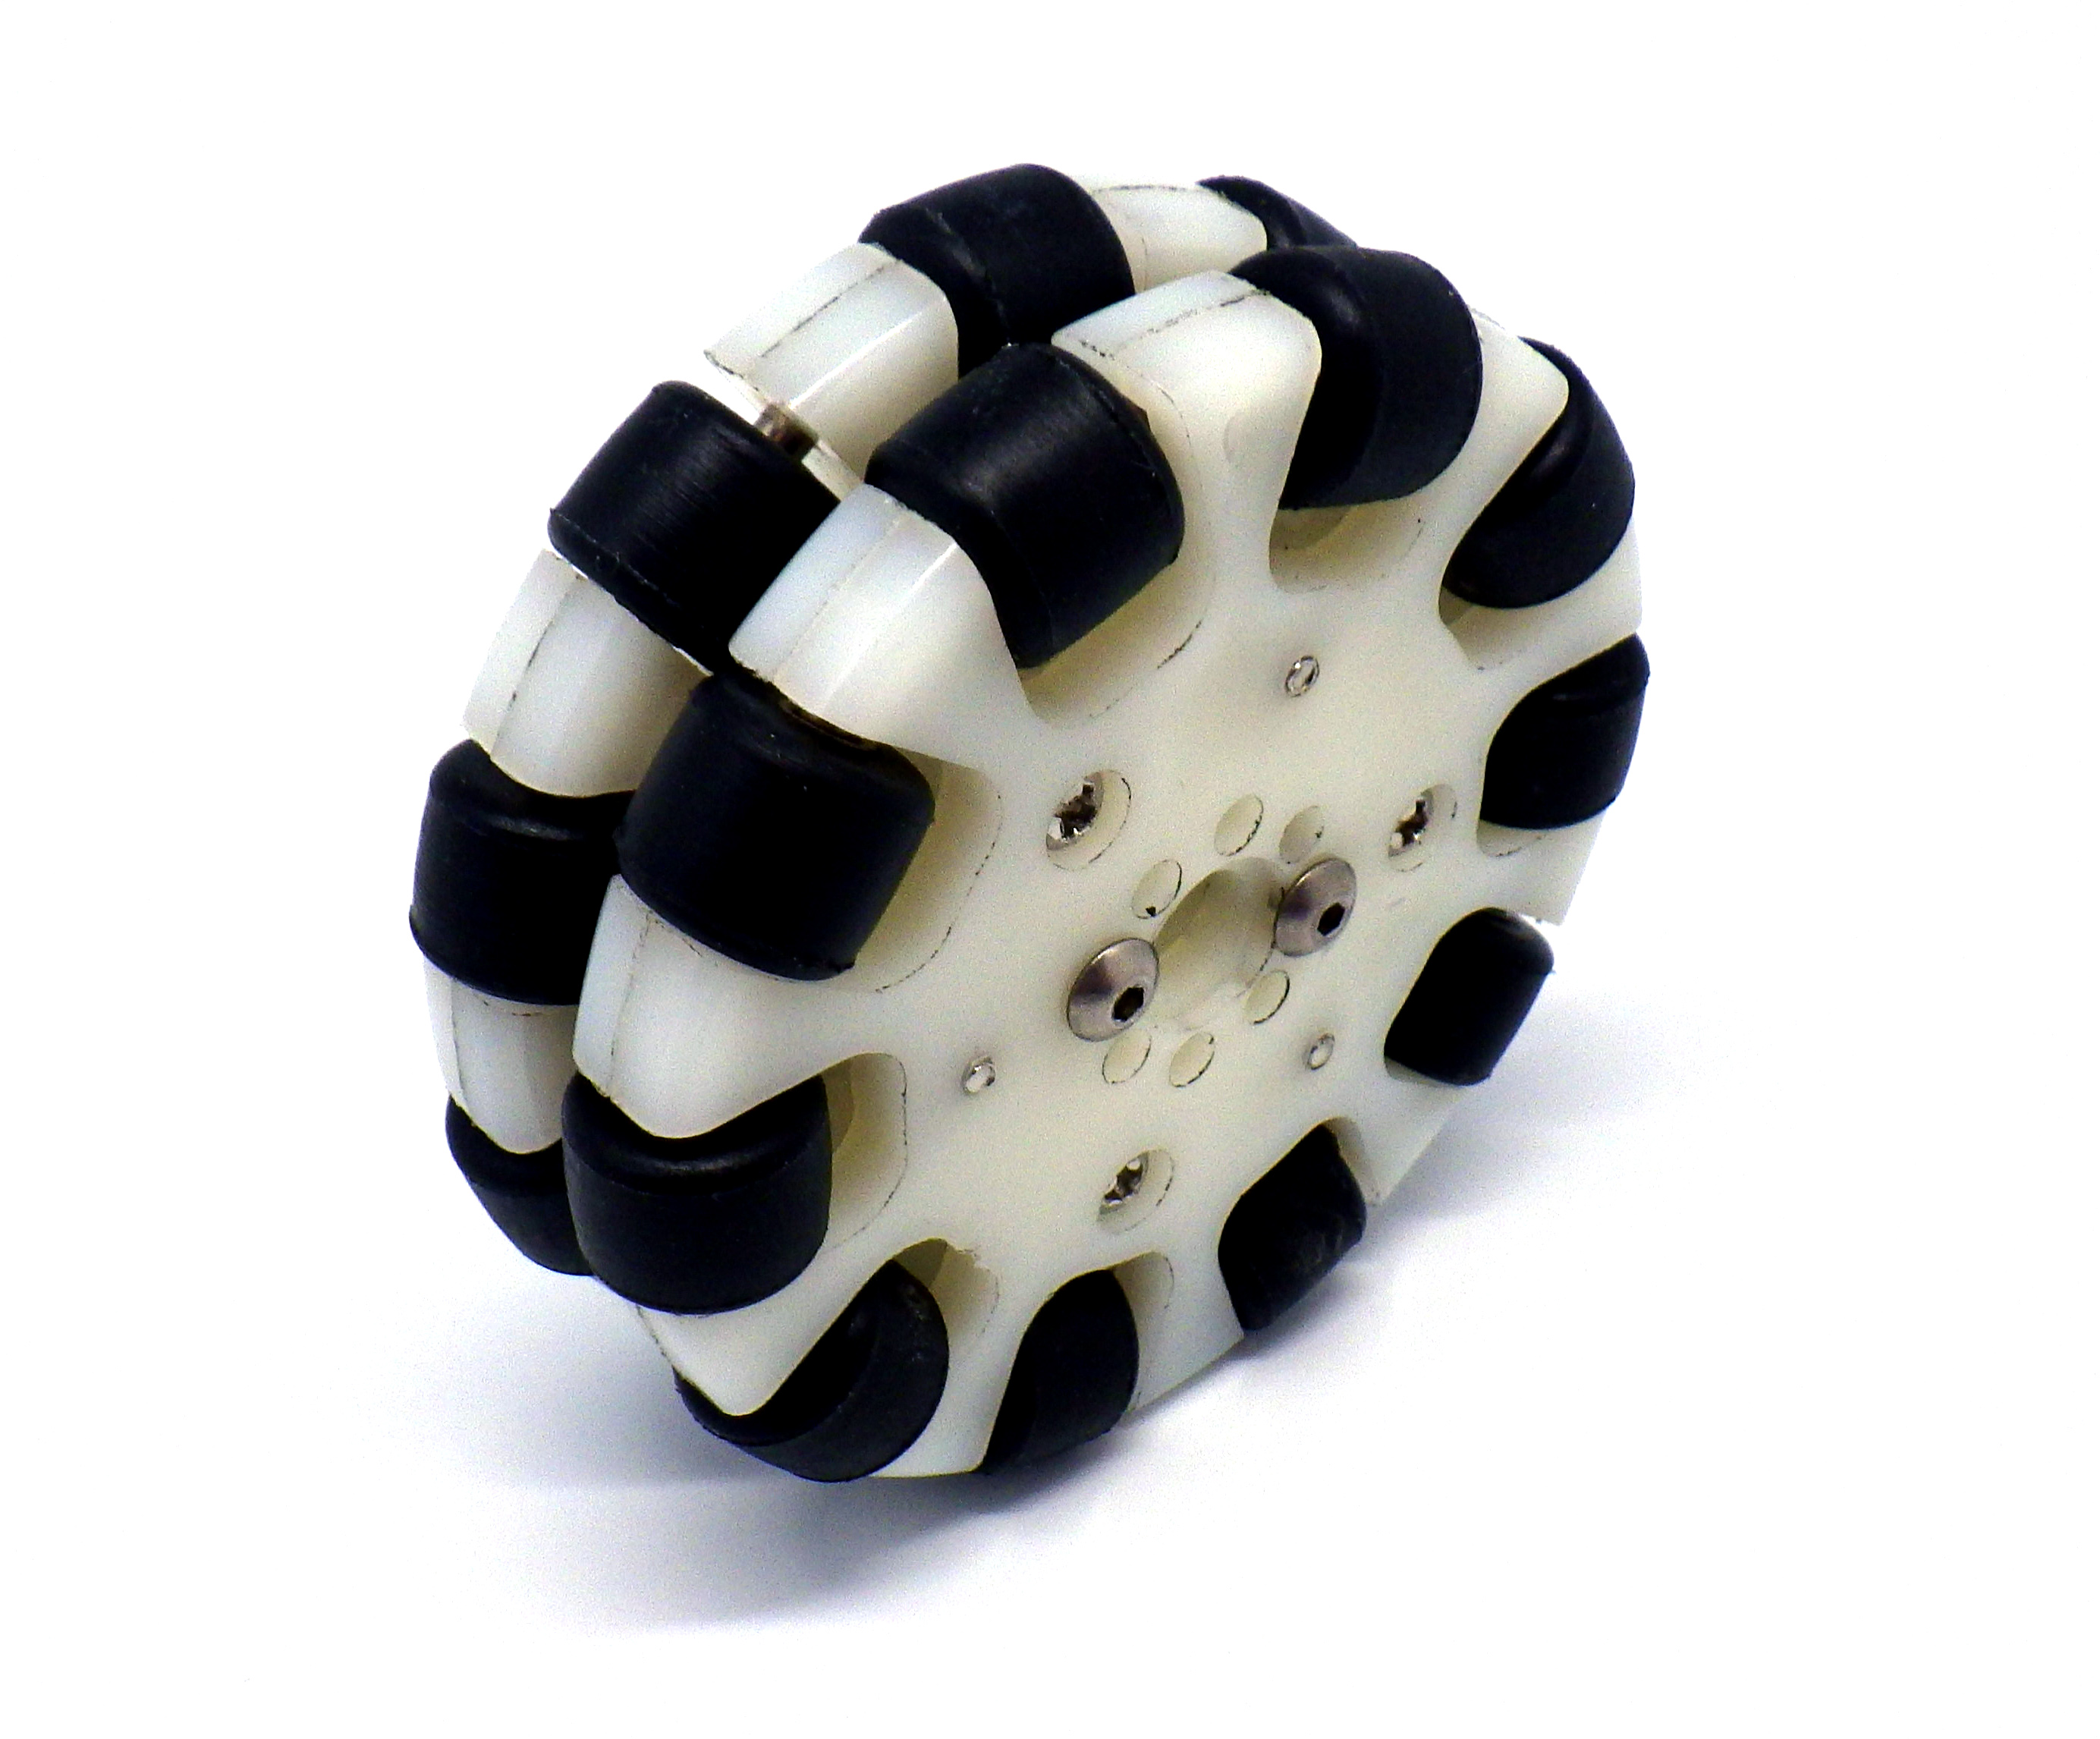
\includegraphics[width=0.45\textwidth]{omni-dir-wheel.jpg}
\caption{Roda sueca}\label{fig.swheel}
\end{minipage}
\hspace{\fill}
\begin{minipage}{.45\textwidth}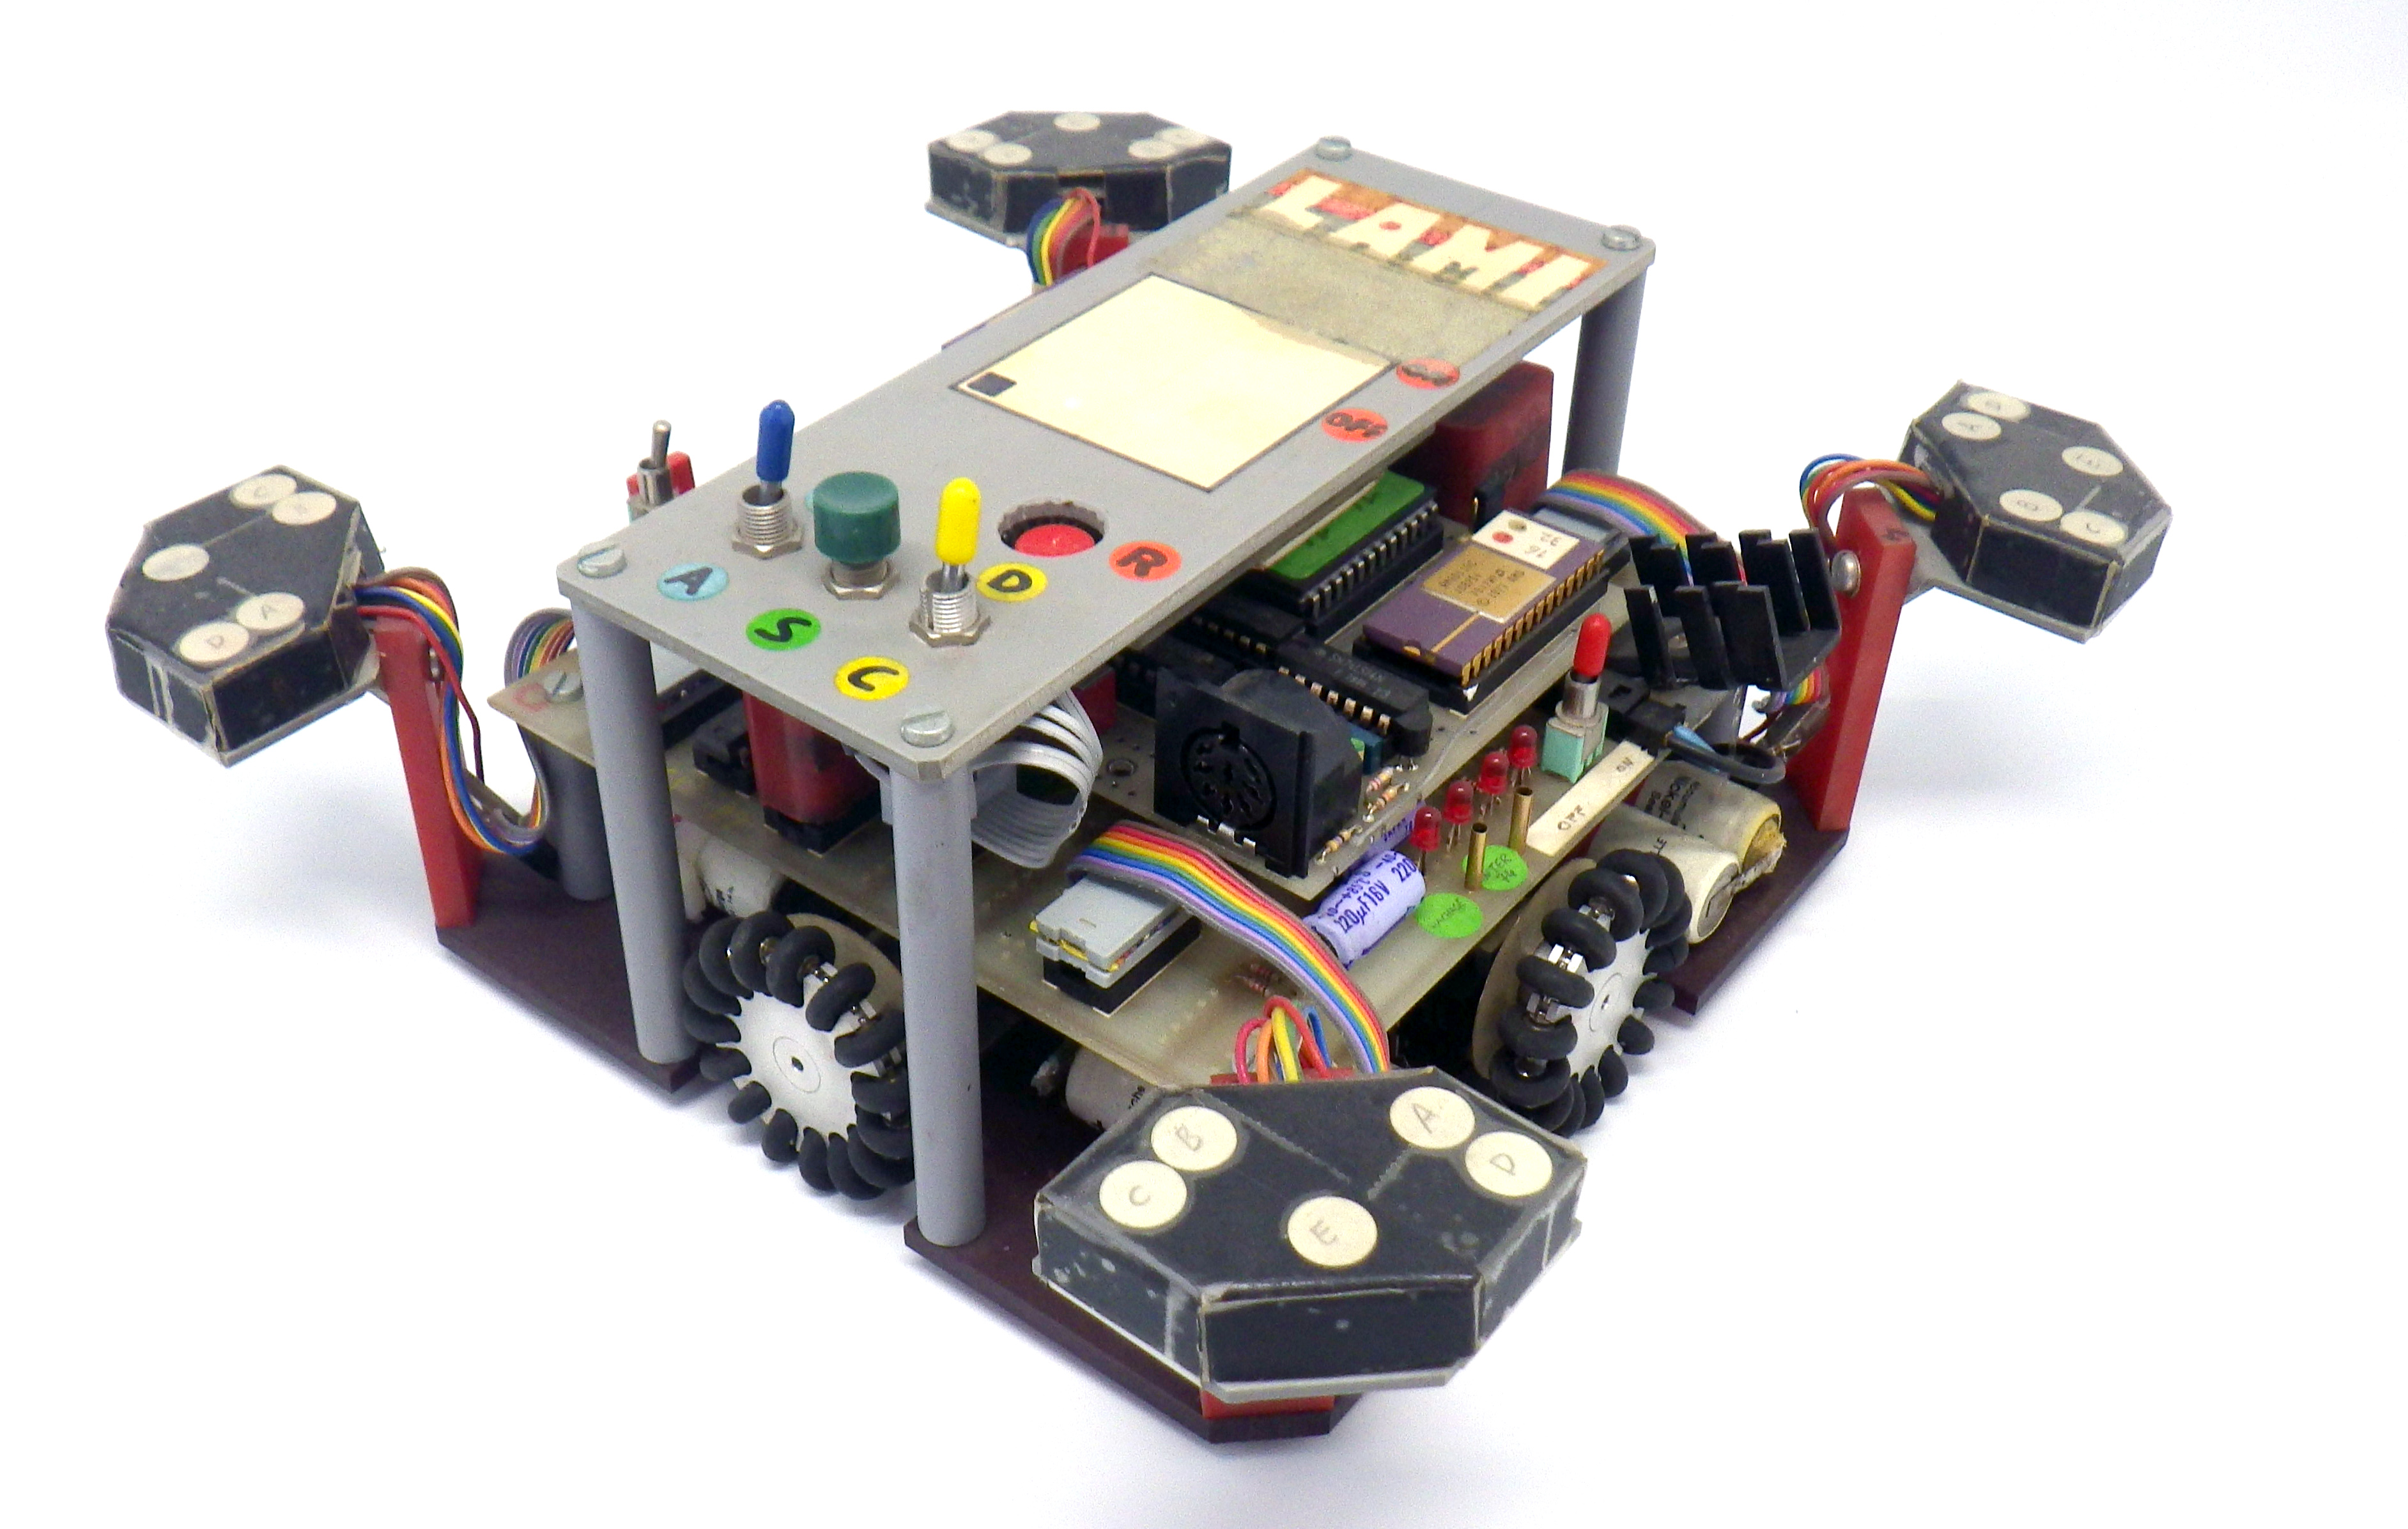
\includegraphics[width=0.5\textwidth]{omnirobot.jpg}
\caption{Robô omnidirecional (Cortesia LAMI-EPFL)}\label{fig.omni-robot}
\end{minipage}
\end{figure}


%\begin{figure}
%\subfigures
%\leftfigure
%{
%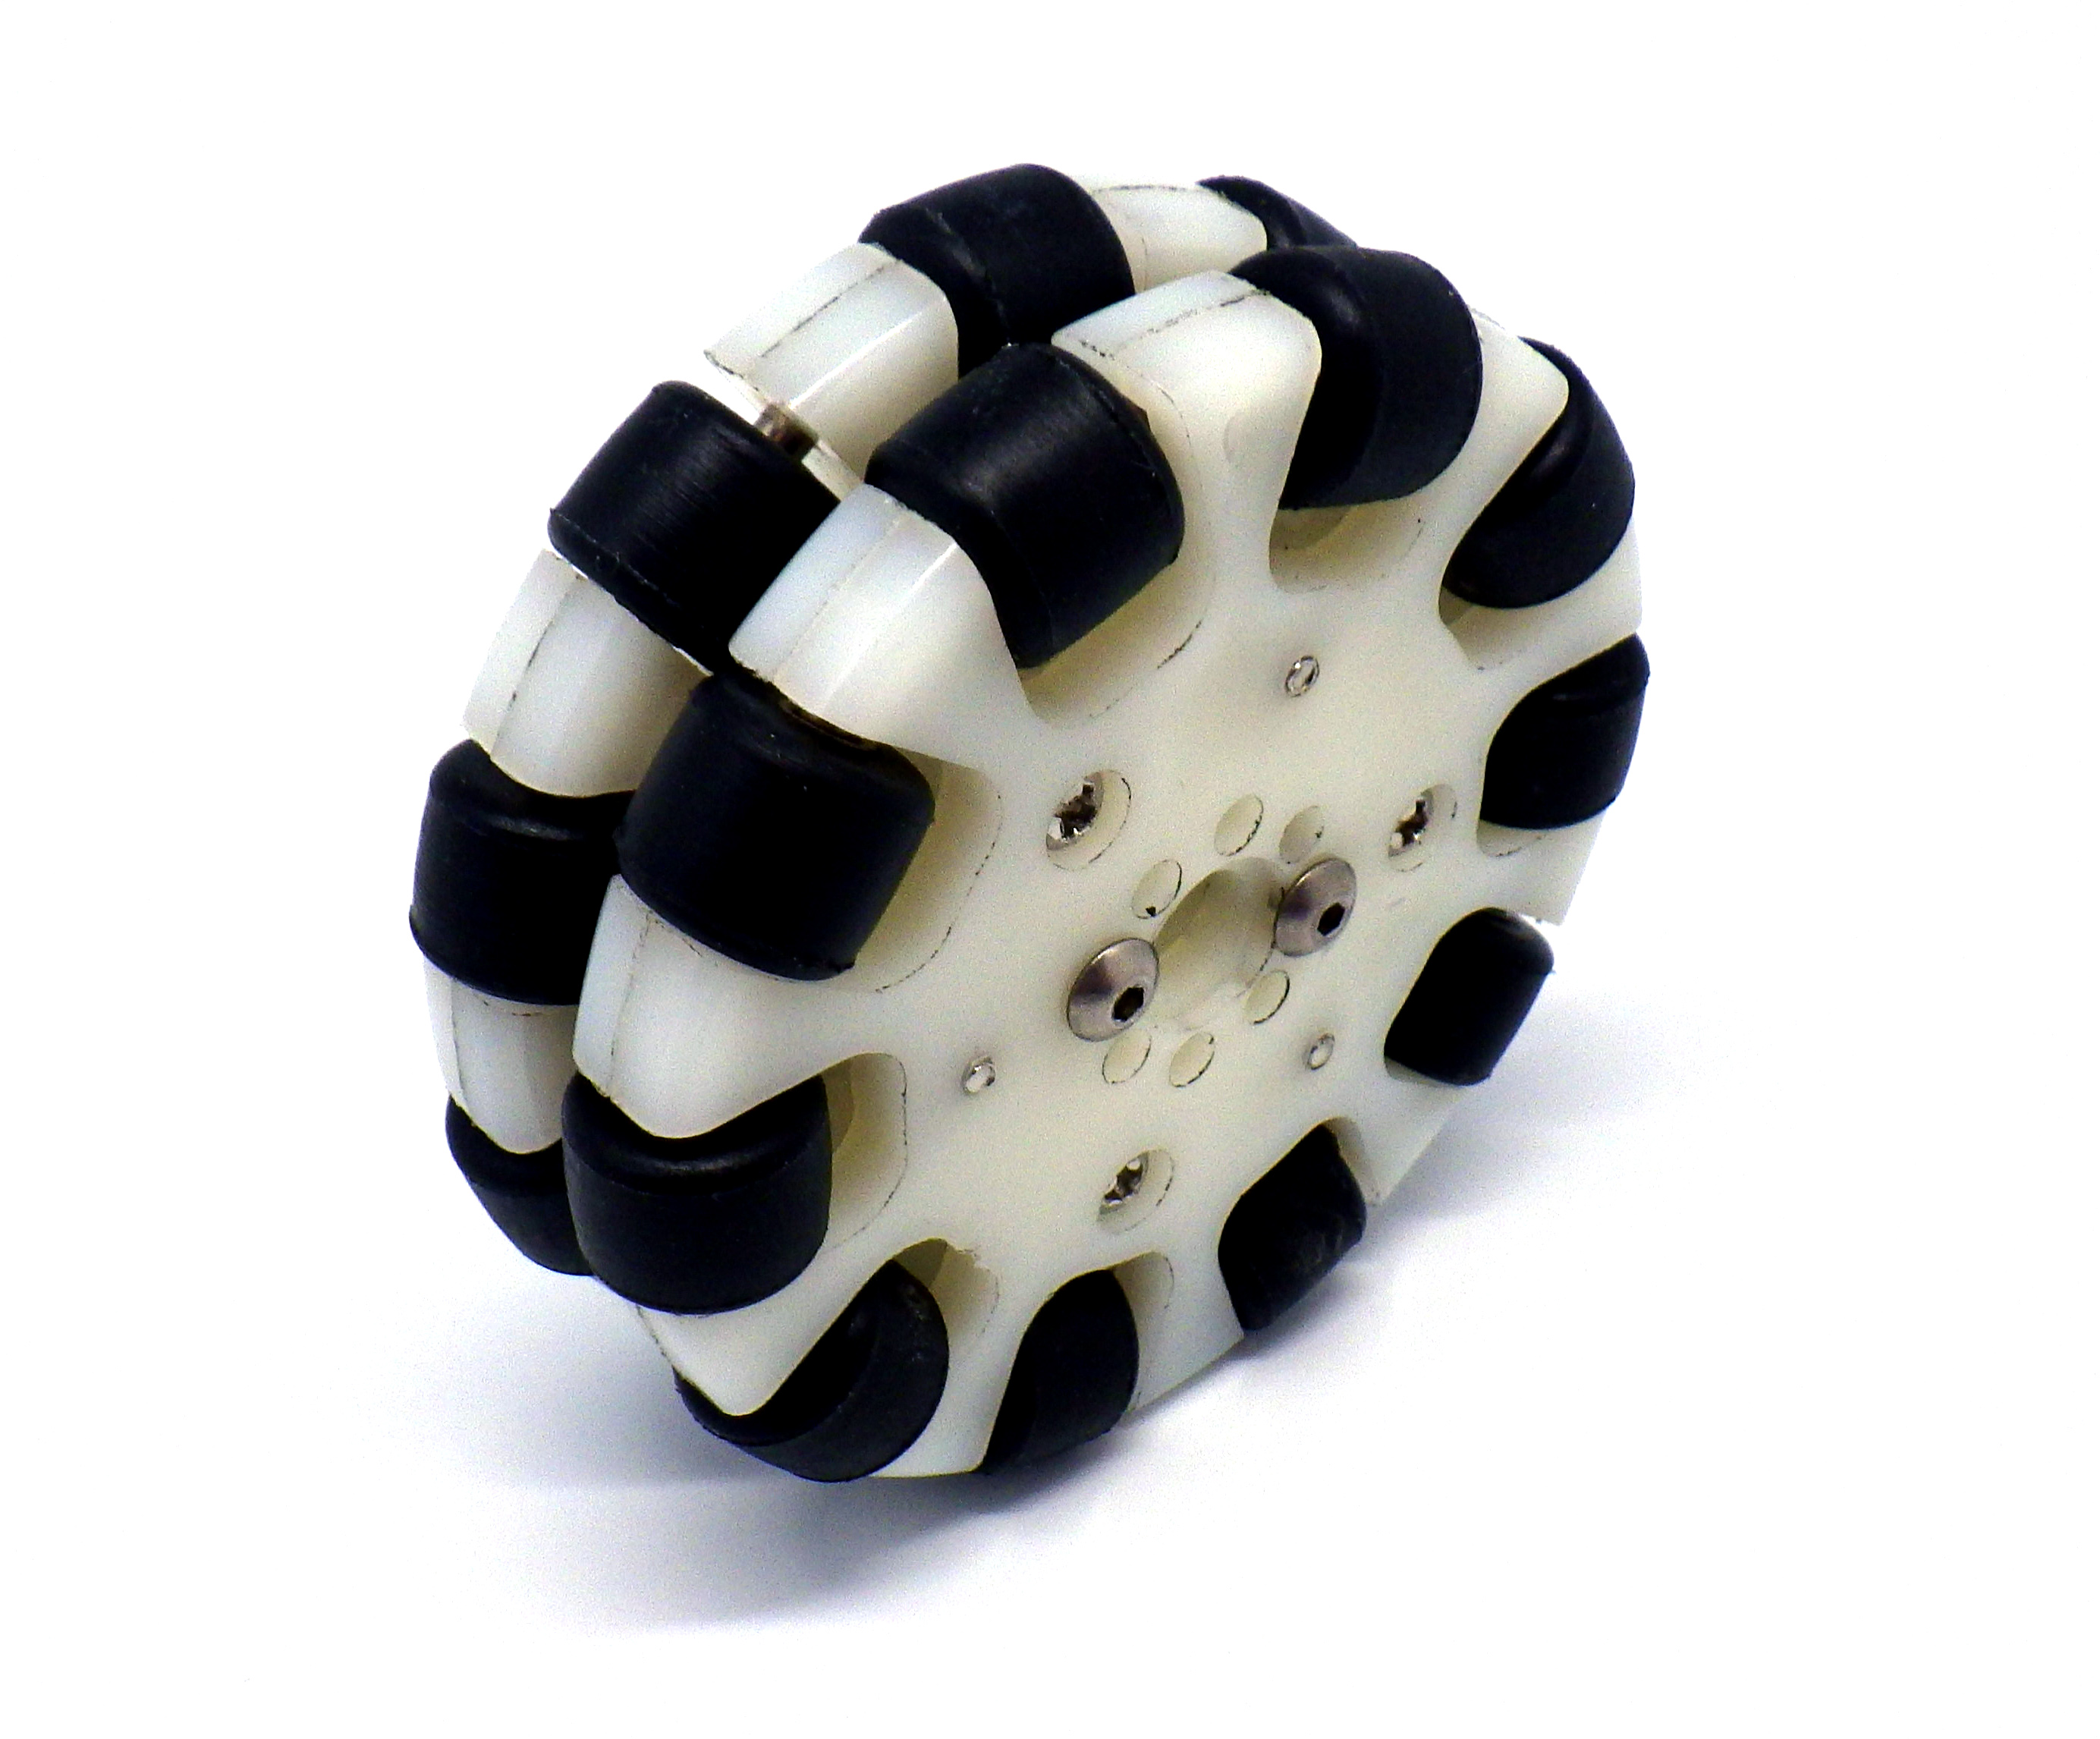
\includegraphics[width=0.45\textwidth]{omni-dir-wheel.jpg}
%}
%\hspace{\fill}
%\rightfigure
%{
%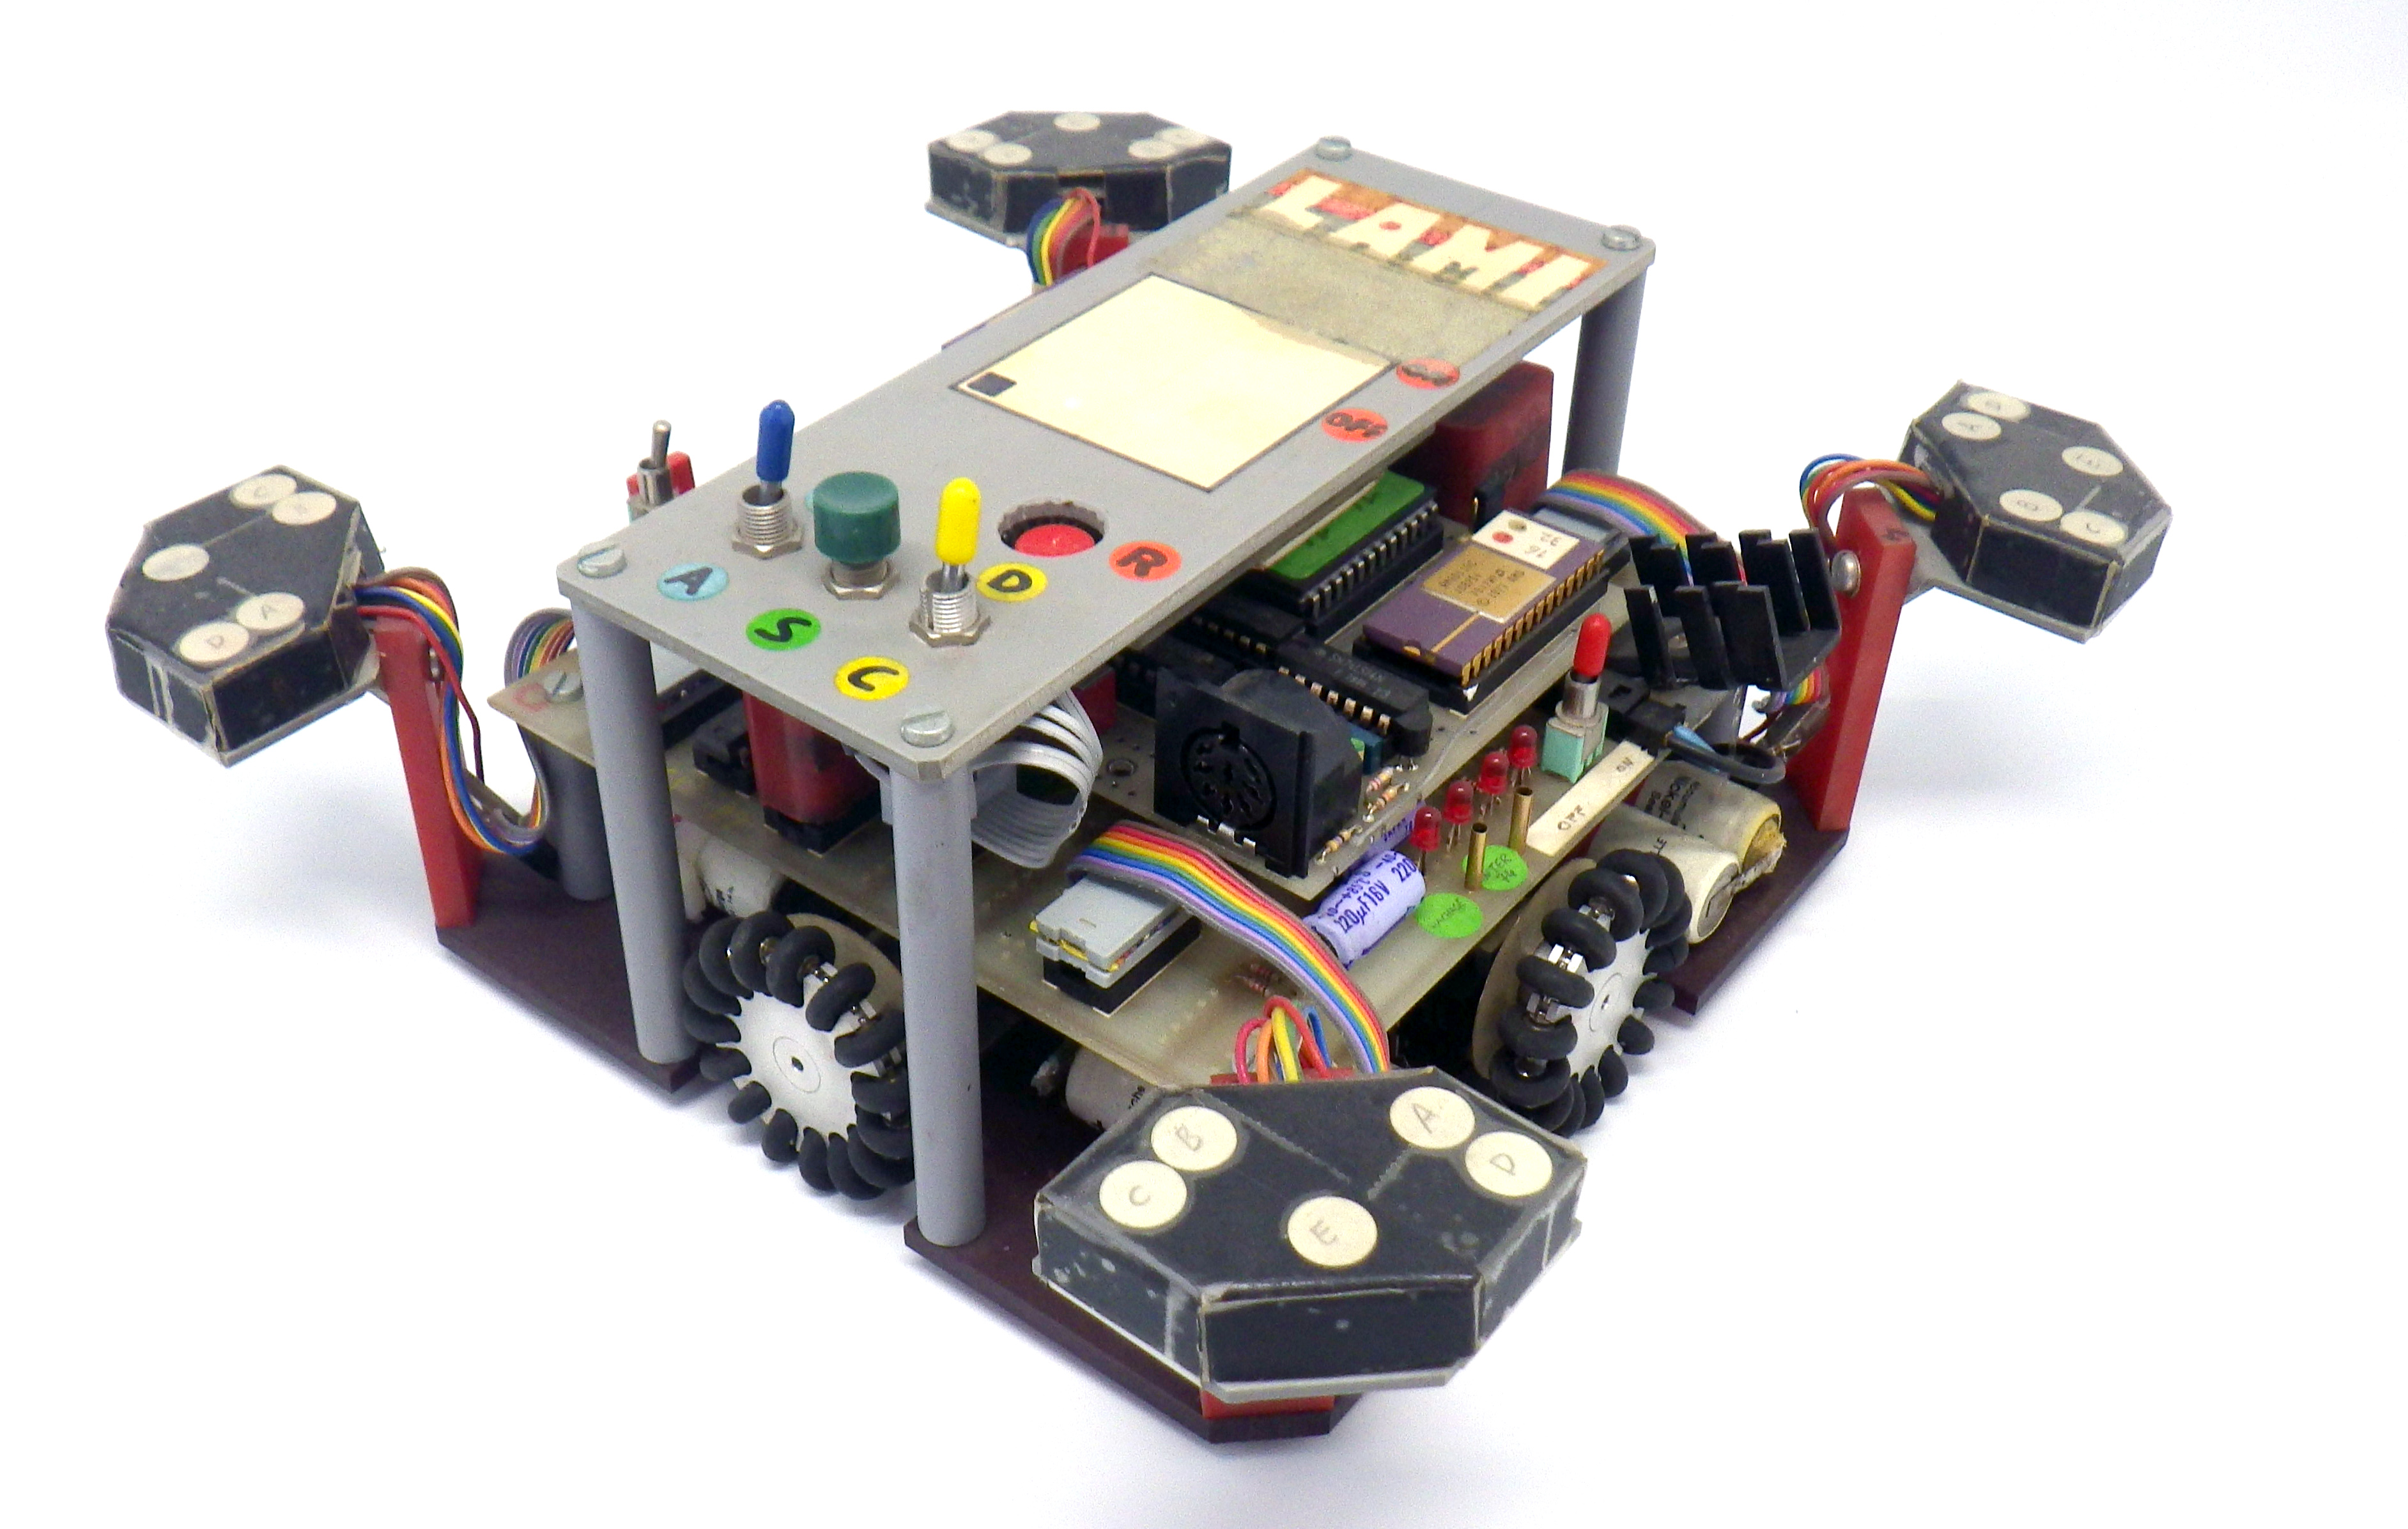
\includegraphics[width=0.5\textwidth]{omnirobot.jpg}
%}
%\leftcaption{Swedish wheel}\label{fig.swheel}
%\rightcaption{Omnidirectional robot (Courtesy LAMI-EPFL)}\label{fig.omni-robot}
%\end{figure}

Os robôs móveis que podem acessar diretamente os três DoF ($\delta_m=3$) são chamados de \emph{robôs omnidirecionais}. A figura~\ref{fig.omni-robot} mostra um robô omnidirecional construído com quatro rodas suecas. Os dois pares de rodas em lados opostos do robô podem mover diretamente o robô para a esquerda, direita, para frente e para trás. Esta configuração é redundante, mas muito fácil de controlar. Para evitar redundância, a maioria dos robôs omnidirecionais tem três rodas suecas montadas a um ângulo de $120^\circ$ uma da outra (Fig.~\ref{fig.omni3}). Esta configuração tem $\delta_m=3$ mas não é fácil de controlar usando as conhecidas coordenadas $x,y$.

\begin{figure}
\begin{center}
\begin{tikzpicture}[scale=0.8]
% Draw body of robot
\draw[fill,gray!20] (0,0) circle [radius=50pt];
% Draw three Swedish wheels
\foreach \r/\x/\y in {0/0/0,120/0cm/0cm,-120/0cm/0cm} {
	\begin{scope}[xshift=\x,yshift=\y,rotate=\r]
		% Draw axle
		\draw[thick,fill,gray] (-3,-0.1) rectangle +(-.5,.2);
		% Draw motor
		\draw[thick] (-3,-.5) rectangle +(2,1);
		% Draw wheel
		\draw[rounded corners,thick,fill=gray!20] (-4,-1) to [bend right=10] ++(.5,0)
		       -- ++(0,2) to [bend right=10] ++(-.5,0) -- cycle;
		\foreach \i in {-.8,-.2,.4} {
		  \draw[rounded corners,fill=gray] (-3.85,\i) rectangle +(.2,.4);
	  }
	\end{scope}
}
% Draw axes
\foreach \r/\x/\y/\len in {60/0/0/4.5cm,180/0cm/0cm/6cm,-60/0cm/0cm/4.5cm} {
	\begin{scope}[xshift=\x,yshift=\y]
	  \draw[raxis] (0,0) -- +(\r:\len);
  \end{scope}
}
\draw[->] (-3.75,1) -- +(0,.5) node[right] {\p{movimento atuado}};
\draw[->,thick] (-4,0) -- +(-1,0) node[above,xshift=-2mm] {\p{movimento livre}};
\node[xshift=-1.6cm,yshift=.2cm] at (0,0) {\p{motor}};
\end{tikzpicture}
\end{center}
\caption{Robô omnidirecional com três rodas suecas}\label{fig.omni3}
\end{figure}

Os valores relativos do DoF e do DoM de um robô definem o conceito de movimento holonômico. Um robô tem \emph{movimento holonômico} se $\delta_m = \#\textrm{DoF}$ e tem um movimento {não-holonômico} se $\delta_m < \#\textrm{DoF}$. Um robô holonômico como o da Fig.~\ref{fig.omni-robot} pode controlar diretamente todos os seus DoF sem manobras difíceis. A Figura~\ref{fig.parallel-omni} mostra como é fácil para o robô omnidirecional com rodas suecas (Fig.~\ref{fig.omni3}) realizar o estacionamento paralelo.

\begin{figure}
\begin{center}
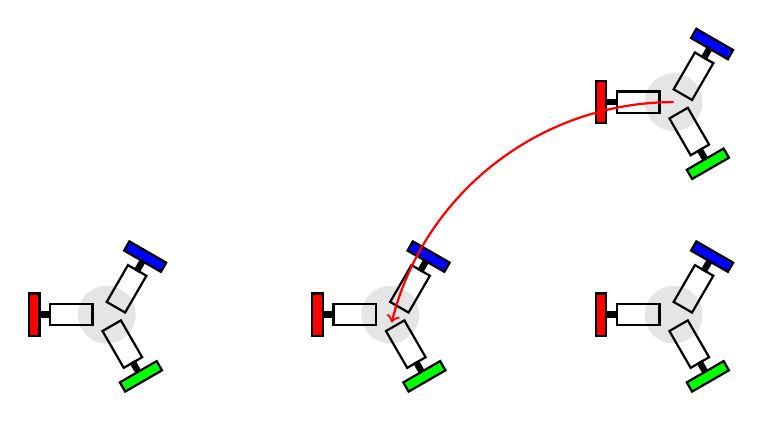
\begin{tikzpicture}[scale=.9]
\foreach \a/\b in {0/0,-40mm/-30mm,-80mm/-30mm,0/-30mm} {
	\draw[fill,gray!20] (\a,\b) circle [radius=4mm];
	\foreach \r/\x/\y/\color in {0/-8mm/-1.5mm/red,120/5mm/-6mm/green,-120/3mm/7mm/blue} {
		\begin{scope}[xshift=\x+\a,yshift=\y+\b,rotate=\r,scale=.3]
			% Draw axle
			\draw[thick,fill,gray] (0,.4) rectangle +(-.5,.2);
			% Draw motor
			\draw[thick] (0,0) rectangle +(2,1);
			% Draw wheel
			\draw[thick,fill=\color] (-1,-.5) to ++(.5,0)
	       -- ++(0,2) to ++(-.5,0) -- cycle;
		\end{scope}
	}
}
\draw[thick,red,->] (0,0) arc (90:166:41mm);
\end{tikzpicture}
\end{center}
\caption{Estacionamento paralelo feito por um robô omnidirecional}\label{fig.parallel-omni}
\end{figure}

Um carro e um robô com acionamento diferencial são não-holonômicos porque seus números de DoM ($\delta_m=1$ e $\delta_m=2$, respectivamente) são inferiores aos seus números de DoF, que são igauis a três. Devido a este grau limitado de mobilidade, estes veículos precisam de manobras de direção mais complexas, por exemplo, para realizar estacionamentos paralelos. Há uma diferença significativa entre os dois veículos. O robô de tração diferencial precisa de três movimentos separados, mas eles são muito simples (Fig.~\ref{fig.parallel-diff}): gire para a esquerda, para trás, para a direita. O carro também precisa de três movimentos separados, mas eles são extremamente difíceis de executar corretamente (Fig.~\ref{fig.parallel-car}). Você tem que estimar onde iniciar a manobra, como fazer cada curva e até onde deve se mover entre as curvas. O DoM superior do robô de acionamento diferencial é vantajoso nesta situação.

\begin{figure}
\begin{minipage}{.45\textwidth}
\begin{tikzpicture}
\pic[scale=.5] at (-14mm,-4mm) { robot };
\pic[scale=.5] at (18mm,-4mm) { robot };
\pic[scale=.5] at (2mm,15mm) { robot };
\pic[rotate=90,scale=.5] at (2mm,15mm) { robot };
\pic[scale=.5] at (2mm,-4mm) { robot };
\pic[rotate=90,scale=.5] at (2mm,-4mm) { robot };
\draw[->,thick,green!60!black] (2mm,10mm) -- +(0,-6mm);
\draw[thick,red,->] (2mm,-4mm) arc (180:90:5mm);
\draw[thick,blue,->] (2mm,15mm) arc (0:90:5mm);
\end{tikzpicture}
\caption{Estacionamento paralelo para um robô de acionamento diferencial não-holonômico}\label{fig.parallel-diff}
\end{minipage}
\hspace{\fill}
\begin{minipage}{.45\textwidth}
\begin{tikzpicture}
\pic[scale=.5] at (-14mm,-4mm) { car };
\pic[scale=.5] at (18mm,-4mm) { car };
\pic[scale=.5] at (20mm,15mm) { car };
\draw[thick,red,->] (18mm,15mm) arc (90:180:10mm);
\draw[thick,blue,->] (8mm,6mm) arc (0:-90:10mm);
\draw[thick,green!60!black,->] (-1mm,-4mm) -- (12mm,-4mm);
\end{tikzpicture}
\caption{Estacionamento paralelo para um carro não-holonômico}\label{fig.parallel-car}
\end{minipage}
\end{figure}


%\begin{figure}
%\subfigures
%\leftfigure{
%\begin{tikzpicture}
%\pic[scale=.5] at (-14mm,-4mm) { robot };
%\pic[scale=.5] at (18mm,-4mm) { robot };
%\pic[scale=.5] at (2mm,15mm) { robot };
%\pic[rotate=90,scale=.5] at (2mm,15mm) { robot };
%\pic[scale=.5] at (2mm,-4mm) { robot };
%\pic[rotate=90,scale=.5] at (2mm,-4mm) { robot };
%\draw[->,thick,green!60!black] (2mm,10mm) -- +(0,-6mm);
%\draw[thick,red,->] (2mm,-4mm) arc (180:90:5mm);
%\draw[thick,blue,->] (2mm,15mm) arc (0:90:5mm);
%\end{tikzpicture}
%}
%\hspace{\fill}
%\rightfigure{
%\begin{tikzpicture}
%\pic[scale=.5] at (-14mm,-4mm) { car };
%\pic[scale=.5] at (18mm,-4mm) { car };
%\pic[scale=.5] at (20mm,15mm) { car };
%\draw[thick,red,->] (18mm,15mm) arc (90:180:10mm);
%\draw[thick,blue,->] (8mm,6mm) arc (0:-90:10mm);
%\draw[thick,green!60!black,->] (-1mm,-4mm) -- (12mm,-4mm);
%\end{tikzpicture}
%}
%\leftcaption{Parallel parking for a non-holonomic differential drive robot}\label{fig.parallel-diff}
%\rightcaption{Parallel parking for a non-holonomic car}\label{fig.parallel-car}
%\end{figure}

\begin{framed}
\act{Movimento holonômico e não-holonômico}{holonomic}
\begin{itemize}
\item Olhe novamente para o robô móvel que é limitado apenas ao movimento rotacional (Fig.~\ref{fig.rot-dof}). Quantos graus de mobilidade $\delta_m$ ele possui? É holonômico ou não?
\item O Fig.~\ref{fig.wallcleaning} mostra um robô para a limpeza de paredes de um edifício. Há duas âncoras das quais descem os cabos, passando hastes fixadas ao corpo do robô e depois pelos guinchos alimentados pelas rodas do robô. Ao enrolar e desenrolar os cabos, o robô se move para cima e para baixo da parede. Entretanto, se os dois motores não fizerem com que as rodas se movimentem precisamente à mesma velocidade de rotação, o robô irá balançar de um lado para o outro. Quantos DoF e quantos DoM este robô tem? É ou não holonômico?
\end{itemize}
\end{framed}


\begin{figure}
\begin{center}
\begin{tikzpicture}[scale=1.2]
% Robot
\pic[rotate=90,scale=1.3] at (0,0) { robot };
% Left and right
\foreach \sign in {1,-1} {
  % Winch
  \draw (\sign*8.5mm,-1mm) rectangle +(\sign*3mm,2mm);
  \draw[fill] (\sign*11.5mm,-2mm) rectangle +(\sign*1mm,4mm);
  % Cable on winch
  \foreach \x in {9mm,9.5mm,10mm,10.5mm,11mm} {
    \draw[red] (\sign*\x,-1mm) -- +(0mm,2mm);
  }
  % Cable
  \draw[red,thick] (\sign*10mm,0mm) -- (\sign*10.8mm,18.5mm) -- (\sign*30mm,45mm);
  % Eyes
  \draw (\sign*10.8mm,18.5mm) circle [radius=.8mm];
  % Anchors
  \draw[fill,gray] (\sign*30mm,45mm) circle [radius=1mm];
}
\draw[fill,gray] (-.5mm,10mm) rectangle +(1mm,8mm); 
\draw[fill,gray] (-10mm,18mm) rectangle +(20mm,1mm);
\node at (0,45mm) {\p{âncoras}};
\draw[->] (6mm,45mm) -- +(20mm,0);
\draw[->] (-6mm,45mm) -- +(-20mm,0);
\begin{scope}[yshift=5mm]
\node at (-22mm,0mm) {\p{guincho}};
\node at (22mm,0mm) {\p{guincho}};
\draw[->] (-18mm,0mm) -- +(5mm,-2mm);
\draw[->] (18mm,0mm) -- +(-5mm,-2mm);
\end{scope}
\draw[raxis] (-18mm,0mm) -- (18mm,0mm);
\end{tikzpicture}
\end{center}
\caption{Robô para a limpeza de uma parede}\label{fig.wallcleaning}
\end{figure}

\section{Sumário}

Um robô móvel como um carro que dirige sozinho ou um explorador de Marte não terá pontos de referência sempre disponíveis para navegação. A odometria é usada para levar o robô até as proximidades de seu objetivo sem referência ao meio ambiente. O robô estima sua velocidade e velocidade de rotação a partir da potência aplicada a seus motores. A odometria pode ser melhorada usando encoders de roda para medir o número de rotações das rodas, em vez de inferir a velocidade a partir da potência do motor. A mudança na posição de um robô barato movendo-se em linha reta pode ser computada multiplicando-se a velocidade pelo tempo. Se o robô estiver girando, cálculos trigonométricos são necessários para calcular a nova posição e orientação. Mesmo com encoders de roda, a odometria está sujeita a erros que podem ser muito grandes se o erro estiver no orientação.

A navegação inercial utiliza acelerômetros e giroscópios para melhorar a precisão da odometria. A integração da aceleração dá velocidade e a integração da velocidade angular dá a orientação. Os sistemas microeletromecânicos tornaram a navegação inercial suficientemente barata para uso em robótica.

O número de graus de liberdade (DoF) de um sistema é o número de dimensões nas quais ele pode se mover - até três dimensões em uma superfície e até seis dimensões no ar ou debaixo d'água - mas um robô pode ser obrigado a ter menos do que o número máximo de DoF. Uma consideração adicional é o número e a configuração dos atuadores de um robô que definem seu grau de mobilidade. Se o DoM for igual ao número de DoF, o robô é holonômico e pode se mover diretamente de uma pose para outra, embora possa ser difícil de controlar. Se o DoM for menor que o número de DoF, o robô é não-holonômico; ele não pode mover-se diretamente de uma pose para outra e exigirá manobras complexas para realizar algumas tarefas.

\section{Leitura adicional}

Um tratamento matemático detalhado dos erros de odometria em duas dimensões é dado em \cite[Sect.~5.24]{siegwart}. Para uma visão geral da navegação inercial, veja em \cite{king,oxford}. Livros didáticos avançados sobre robótica apresentam o conceito de holonomia \cite{correll,craig,siegwart,spong}.
